\documentclass{tudelft-report}
% Options:
% dutch - for a Dutch report
% print - for a print version
% draft - for locating problem areas
% nativefonts - override automatic font selection

\usepackage{natbib}
\usepackage{lipsum}
\usepackage{changes}
\usepackage{csquotes}
\usepackage{setspace}
\usepackage{mathtools}
\usepackage{todonotes}
\usepackage{float}
\usepackage{multicol}
\usepackage{pifont}
\usepackage{hyperref}
\usepackage{xcolor}
\usepackage{listings}
\usepackage{caption}
\usepackage{subcaption}
\usepackage{booktabs}
\usepackage{enumitem}
\definecolor{green}{RGB}{50,205,50}
\definecolor{red}{RGB}{178,34,34}
\definecolor{orange}{RGB}{255,165,0}
\newcommand{\itemcolor}[1]{% Update list item colour
  \renewcommand{\makelabel}[1]{\color{#1}\hfil ##1}}

\begin{document}

%% Use Roman numerals for the page numbers of the title pages and table of
%% contents.
\frontmatter

\newcommand\TITLE{\fontsize{40}{60}\selectfont}

%% Uncomment following 19 lines for a cover with a picture on the lower half only
\title[tudelft-white]{\TITLE{FBase:}}
\subtitle[tudelft-cyan]{\Huge{Trustworthy code module execution}\\}
\author[tudelft-white]{M.J.G. Olsthoorn}
\affiliation{Technische Universiteit Delft}
\coverimage{cover.jpg}
\covertext[tudelft-white]{
    \textbf{Cover Text}
}
\makecover[whitelogo]

%% Include an optional title page.
\begin{titlepage}
	
	
	\begin{center}
		
		%% Insert the TU Delft logo at the bottom of the page.
		
		%% Print the title in cyan.
		{\makeatletter
			\largetitlestyle\fontsize{64}{94}\selectfont\@title
			%\largetitlestyle\color{tudelft-cyan}\Huge\@title
			\makeatother}
		
		%% Print the optional subtitle in black.
		{\makeatletter
			\ifx\@subtitle\undefined\else
			\bigskip
			{\tudsffamily\fontsize{22}{32}\selectfont\@subtitle}    
			%\titlefont\titleshape\LARGE\@subtitle
			\fi
			\makeatother}
		
		\bigskip
		\bigskip
		
		by
		%door
		
		\bigskip
		\bigskip
		
		%% Print the name of the author.
		{\makeatletter
			%\largetitlefont\Large\bfseries\@author
			\largetitlestyle\fontsize{26}{26}\selectfont\@author
			\makeatother}
		
		\bigskip
		\bigskip
		
		to obtain the degree of Master of Science
		%ter verkrijging van de graad van Master of Science
		
		at the Delft University of Technology,
		%aan de Technische Universiteit Delft,
		
		to be defended publicly on Tuesday December 1, 2019 at 10:00 AM.
		%in het openbaar de verdedigen op dinsdag 1 januari om 10:00 uur.
		
		\vfill
		
		\begin{tabular}{lll}
			Student number: & 4294882 \\
			Project duration: & \multicolumn{2}{l}{March 1, 2018 -- December 1, 2019} \\
			Thesis committee: & Dr.\ ir.\  J.A.\ Pouwelse, & TU Delft, supervisor \\
			& Dr.\ J.S.\ Rellermeyer, & TU Delft \\
			& Dr. A. Katsifodimos, & TU Delft
		\end{tabular}
		%% Only include the following lines if confidentiality is applicable.
		
		\bigskip
		\bigskip
		%\emph{This thesis is confidential and cannot be made public until December 31, 2013.}
		%\emph{Op dit verslag is geheimhouding van toepassing tot en met 31 december 2013.}
		
		\bigskip
		\bigskip
		An electronic version of this thesis is available at \url{http://repository.tudelft.nl/}.
		%\\[1cm]
		
		%\centering{
\includegraphics{cover/logo_black}}
		
		
	\end{center}
	
	\begin{tikzpicture}[remember picture, overlay]
	\node at (current page.south)[anchor=south,inner sep=0pt]{
		
\includegraphics{cover/logo_black}
	};
	\end{tikzpicture}
	
\end{titlepage}


\chapter*{Preface}
\setheader{Preface}

Preface\ldots

\begin{flushright}
{\makeatletter\itshape
    \@author \\
    Delft, November 2019
\makeatother}
\end{flushright}


\chapter*{Abstract}
\setheader{Abstract}

The abstract should contain a brief overview of the research and the most important results
\tableofcontents

%% Use Arabic numerals for the page numbers of the chapters.
\mainmatter
    \chapter{Introduction}

%intro to title and topic (start broad and work down to more detail. Try to captivate the reader)
For decades software re-use has been seen as the holy grail of software development. Even in the eighties, papers were already written about this topic~\cite{standish1984essay}. Throughout the years, more and more research has been done on the benefit of re-usable software~\cite{jacobson1997software}. Studies have also been performed on how to re-use software in practice~\cite{reifer1997practical}. But up until recently, there was more discussion about software re-use than actual software re-use. Even though most software uses the same blocks of code over and over again, almost all software is built from the ground up~\cite{frakes2005software}. Today, this situation is completely different. Nowadays, almost every application re-uses software in the form of software dependencies. However, this re-use pattern is starting to become unchecked. The shift to re-usable software has happened so quickly, the risks associated with choosing the right dependencies are often overlooked~\cite{cox2019surviving}. 

%Describe the topic and scope of your research
\section{Code Evolution}
% Monolithic and libraries
Over the years, the way we use code has evolved with the changing need of the users and society as a whole~\cite{rajlich2014software}. This evolution started with specific applications written for each use case and each platform it had to run on. These so called monolithic applications took a lot of time to develop and could not be re-used. To reduce this time, system libraries were built to make it possible to run these applications on similar platforms. This abstraction layer, however, was still limited to broader types of platforms e.g. Linux, Unix, Windows. These shared system libraries could now be maintained and distributed separately. This led to easier development and applications that could be used on more systems.

% Example
The Debian package system is a good example of this evolution. It made it possible for code that was meant to be used as a library to be packaged separately for both system and user code. This allowed applications to indicate which library would be required for that application and the system would make sure it is available to the application. This possibility allowed these applications to be developed faster. ~\cite{zacchiroli2011debian}

% Plug-ins
% In computing, a plug-in (or plugin, add-in, addin, add-on, or addon) is a software component that adds a specific feature to an existing computer program. When a program supports plug-ins, it enables customization. to enable third-party developers to create abilities which extend an application, to support easily adding new features, to reduce the size of an application, to separate source code from an application because of incompatible software licenses.

These new shared code libraries provided a lot of benefits and speed to application developers, but to improve the ecosystem further a new step had to be made. At this point when applications were distributed they were static. There was no option to adapt the application to include features that the user would like to see. Also, users that wanted to add their own functionality had to go through the developers to accomplish this. To solve this, the larger applications began to include plug-in systems. A plug-in system allows specific functionality to be added to an existing computer program. This enabled customization of applications, making it possible to reduce the size of the core application or separating source code because of incompatible licenses. This paradigm allowed the rapid development of extra features by both developers and the users of the application.

% Example
A well known example of a program with a plugin system is Winamp. The Winamp developers used a plug-in system to provide users with a customizable package that could serve each user's preference~\cite{nullsoft1999winamp}. A large community formed around the application with different plug-ins for every imaginable feature~\cite{winampcommunity}. This community building gave an incentive for other applications to implement similar plug-in systems.

% Cross-platform applications
% software written in an interpreted language or pre-compiled portable bytecode for which the interpreters or run-time packages are common or standard components of all platforms
Eventually programming languages were created that allowed the development of cross-platform applications that could be run on all common platforms. This eliminated the need to create separate binaries for each individual platform. These applications were either written in an interpreted language, e.g. Python, or in a pre-compiled portable byte-code format for which interpreters exist on all platforms, e.g. Java. In the last decade, a major part of these cross-platform applications have moved towards the web. These new web applications make use of existing cross-compatibility of web technologies, that were designed when the web became universal, that run on all platforms.

%  Code frameworks e.g. Spring, Wordpress, Android
With the development of cross-platform applications, there was also a rise in the availability of code frameworks. A code framework provides particular functionality as part of a larger software platform to facilitate development of software applications. Software with common use-cases could make use of the abstraction provided by these code frameworks to create application-specific software with only limited additional user-written code. These code frameworks can be seen everywhere nowadays. Some examples of code frameworks are: Spring, WordPress, and the Android platform. Spring is a popular code framework for developing applications in Java. WordPress is a web framework that runs more than 25\% of the websites on the internet~\cite{ewer201414}. The Android platform is the underlying framework that allows apps to be created for the Android mobile operating system.

% Micro-services
% collection of loosely coupled services
A more recent concept in the development of software applications is the microservice architecture. This architecture breaks an application up into a collection of loosely coupled services. These services are normally small in size and have one use-case that they were specifically designed for~\cite{thones2015microservices}. This architecture facilitates code re-use on a big scale with platforms like NPM (Node Package Manager) storing over 750.000 JavaScript packages~\cite{npmstatistics}.

\section{Code Re-use}

The constant factor during this code evolution is code re-use. The ability to make development easier and faster by making use of existing solutions already created by a different party.

% We want re-use so badly, yet our failures are spectacular. Almost all major technology trends of the past 20 years touts reuse as the saving grace. Vendors have sold billions of dollars in software through the broken promise of increased reusability. https://dzone.com/articles/reuse-dream-dead
Re-use is software development’s unattainable goal. The ability to put together systems from re-usable elements has long been the ultimate dream. Almost all major software design patterns resolve around extensibility and re-use. Even the majority of architectural trends aim for this concept. Despite many attempts in almost every community, projects using this approach often fail~\cite{reusedreamdead}.
%In general, the more reusable we choose to make a software component, the more difficult that same software component is to use. In the extreme, an infinitely reusable component is infinitely difficult to use. Dealing with the tension between re-use and use is a complex issue, and often, we fail. Largely, the problem has to do with dependencies.
This is often attributed to one big problem: usability. The more reusable we try to make a software component, the more difficult it becomes to work with said component. This is a critical balance that needs to be worked on.

\subsection{Re-usability vs Usability}
%The challenge we run into when attempting to create a highly reusable component is to manage the tension between reusability and useability. In our example above, breaking out the coarse-grained component into fine-grained components makes it more difficult to use each of the resulting fine-grained components. Likewise, creating a lightweight component makes using the component more difficult since the component must be configured each time the component is used.
%
%Fine-grained components have more component dependencies and lightweight components have more context dependencies. Each makes a component more re-usable, but also more difficult to use. The key is to strike a balance, and that is a topic for another day not too far away.

The challenge we face when creating a highly re-usable component is to find this balance between re-usability and usability.

To make a component more re-usable it needs to be broken down in smaller parts, that each handles only one task. Components with multiple tasks are harder to re-use since each application has different use cases and therefore has to modify and maintain there own version of that component. Smaller components that handle only one task can be used as building blocks for bigger components making them easier to re-use, saving developers the need for maintaining their own version. However, to create complex application hundreds of small re-usable components would have to be used creating a problem of itself. How are all these components going to be managed? The largest part of this problem has to do with dependencies~\cite{reusedreamdead}, an additional piece of code a programmer wants to call. Some aspects to think about are:
\begin{itemize}
	\item Is the API (Application Programming Interface) going to stay constant?
	\item How do we deal with breaking changes?
	\item How do we prevent dependency conflicts?
\end{itemize}

\noindent Some of these aspects are already partly being addressed through Semantic versioning~\cite{preston2013semantic}, but most of these are still unsolved today.

The context dependability of a component also greatly affects the balance between re-usability and usability. When a component depends on the context it is running in, it makes it impossible to move it to an different environment that does not have this context. For components to be more re-usable, this context has to be moved from code to configuration. However, if each small component has to be configured each time it is used, the application would become less usable.

Both the granularity and the degree of dependability on the context can improve the re-usability at the cost of usability. The key is to find a balance.

\newpage

\section{Component Terminology} % Modules vs Plug-ins

Two different kinds of reusable components that are often integrated into applications are modules and plug-ins. Since these terms can have a different meaning depending on the application, the interpretation that this work will use is defined below:

\begin{itemize}
	\item \textbf{Modules} are main functionality components that are used to break up the application into smaller subsystems that can more easily be worked on with different/larger teams. Modules can either by re-usable components or tied to the specific application, and should be able to operate independently
	\item 
	% Plug-ins depend on the services provided by the host application and do not usually work by themselves. Conversely, the host application operates independently of the plug-ins, making it possible for end-users to add and update plug-ins dynamically without needing to make changes to the host application
	\textbf{Plug-ins} are components used to extend the main functionality of the application without having to make changes to it. They are often created by the community of the application. The functionality in these plug-ins are often too small or too unique to integrate into the core application. Plug-ins depend on the services provided by the application, they do not operate independently. They are also tied to a specific application and can not be re-used for other applications.
\end{itemize}

\noindent The function of both kinds of components is, however, not different. They both provide extra functionality to the application. It would therefore also make sense to both make them first-class citizens of the application instead of making plug-ins a secondary operator.

This distinction is often made to differentiate between the code of the original authors and code created by third-parties. Plug-ins are most of the time also not reviewed by the original authors of the project.

% https://student.unsw.edu.au/introductions
\section{Research Goal}

% What is done, what is missing?
Over the last couple decades, extensive research has been performed into the field of software re-use. In this period, several survey studies have been done to see what different approaches were used in research literature for creating re-usable software~\cite{krueger1992software}~\cite{frakes2005software}. The surveys tried to make generalizations about the methods used to research if there is a common pattern among them. The approaches mostly centered around re-using code for common use-cases like code frameworks. 

Other studies have worked on designing metrics and models for measuring progress in software re-use to identify the most effective strategies~\cite{frakes1996software}. Morisio et al looked at success and failure factors in software re-use to identify key factors in its adoption~\cite{morisio2002success}. The main cause of failures that they discovered was a lack of commitment by companies and projects.

A more recent study, attempted to build a framework for highly modular and extendable software systems, called Normalized System theory. This theory is based on a theoretical concept called system theory. This theory, however, takes the abstraction of modules to a level that makes it inefficient beyond usage. It takes this approach to make the system more agile. However, without simplicity all agility is lost. ~\cite{de2018enabling}

%Normalized System theory == purist, holy grain and therefore inefficiency beyond usage. Too complex. 

Lehman's laws of software evolution is a law describing the evolution of software. The law describe a balance between forces driving new developments on one hand, and forces that slow down progress on the other hand~\cite{lehman1980programs}~\cite{lehman1997metrics}~\cite{herraiz2013evolution}. One of the forces that slows down the progress of new developments is the ability of developers using the development to understand and easily use the functionality of the development.

%Explain the scientific situation related to your topic - you can include the most important scientific articles and briefly explain them and how they are related to your research. 
% Discuss current situation/gap, explain why further research is necessary
% why (personal interest and interest for general use)
% - Another attempt at holy Grail of software re-usability

In the current research there exits a gap in balance between re-usability and usability. This works tries to fill that gap. Many people have tried solving the problem of software re-use, but it has proven to be a hard problem. There needs to be a trade-off between re-usability and usability.

This thesis focuses its work on developing a framework that continues the progression in the development of re-usable code. It tries to find a balance between the software practices of Today and the impractical concepts of the future.

There have already been many attempts to solve the goal of practical code re-usability. However, these attempts still left some problems open, that this thesis tries to solve. These problems include:

\begin{itemize}
	\item How to find a trade-off between re-usability and usability?
	%\item How to minimize the risk associated with the use of dependencies?
	\item Can we use social trust and crowdsourcing to improve security of libraries
	\item How to ensure dependency availability efficiently and securely?
	% includes updates, trustability
	% NPM packages were deleted, but a lot of applications depended on this dependency
\end{itemize}

%contribution to the field (aim/goal)

%how (structure/method of the research) / methodology
The rest of this document is outlined as follows: Chapter 2 will go further into the problems that this thesis tries to solve. Chapter 3 will discuss the solution proposed to solve the problems mentioned in Chapter 2. Chapter 4 will discuss the proof-of-concept implementation. Chapter 5 will evaluate the proposed framework against existing solutions. We use a concrete use-case driven methodology to advance the cause of software re-usability. 

% - show the viability of our ideas with a non-trivial use-case

\chapter{\label{chap:requirements}Requirements}

% Still no good solution for code re-use

% plugin vs module vs micro-service vs middleware

%validate this with real-world complexity
%our unique requirements: ToDo into a Related Work table (red and green ticks)
%

This work sets out to create a framework for the next evolution of modularized code execution to find a balance between software re-usability and usability. This chapter specifies the requirements that were identified from the background and related work in Chapter~\ref{chap:introduction}. The key property is permission-less code execution at near-zero cost.

%There should be no difference between modules and plug-ins. Each user can also choose which functionality and therefore module they want to run on their instance of the application. This allows users to compose their own desired version of the application. The user can compose larger modules out of smaller ones or fork modules to represent their view on how it should be done. This should create a community around each module that could spark an ecosystem.

%Requirements for our envisioned runtime engine are as follows

The requirements are subdivided into three different categories namely Principles, Trustworthy Code, and Runtime Support.

\section{Principles}

These principles form the foundation of the framework and are necessary to achieve the research aim.

\subsection*{Decentralized}

For the framework to be financially sustainable it needs to be decentralized. In centralized systems, the operating costs of a network are the responsibility of the entity in control of the system. This entity would need to have continued incentive to keep operating the network. In decentralized systems, the operating cost is split across all users of the network. The number of users will scale together with the cost of the network.

Decentralization also increases the reliability of the system as there can be no central infrastructural point of failure that could bring the network down. The system should have no central servers except for bootstrapping.

\subsection*{Self-governing}

The system must be able to run by itself without supervision as there is no parent governing entity. The system should be able to handle all the tasks needed for operating the network.

To be free of external influence, no central entity or central governance can be in control of the network. The network should be owned by everybody and nobody and therefore self-governing.

Since self-governing systems are run by the system itself and its users' input, there is no single owner of the network. If the original author disappears or is mandated to hand over control to another party, the overall system is not affected and can continue to function regardless.

An example of a platform that was taken down by external pressure from lawsuits is Napster, a peer-to-peer music sharing service\cite{mccourt2003creators}. Although Napster used decentralization for file sharing it was still controlled by a central company. This allowed lawsuits to be filed against this company to take down the service.

\section{Trustworthy Code}

%https://harry.garrood.me/blog/malicious-code-in-purescript-npm-installer/
%https://lwn.net/Articles/740157/
%https://blog.cloudflare.com/cloudflare-architecture-and-how-bpf-eats-the-world/
%https://news.ycombinator.com/item?id=19947970
%https://arstechnica.com/information-technology/2018/06/backdoored-images-downloaded-5-million-times-finally-removed-from-docker-hub/

Since this work is proposing a framework that is highly dependent on re-usable code, it is important that the user running the application can trust all its parts. This trust aspect is very important for a code execution ecosystem. There are countless examples of applications being compromised by running untrusted code~\cite{purescript}\cite{docker}.

\subsection*{Open Ecosystem}
For a user to trust the application they want to run, they also need to trust the framework running it. That is why every part of the code execution ecosystem must be open for inspection. Making the source code public allows users or external parties to verify the behavior of the system. 

Next to opening up the framework for inspection, it is also of vital importance that each re-usable component used within the framework can be inspected to increase the trustworthiness of the code.

\subsection*{Crowdsourcing}
DevID is a previous work of the authors of this thesis. It evaluates the possibility of using social trust as a way to increase the trustworthiness of code by using crowdsourced peer-review~\cite{de2019devid}.

Cargo Crev is a cryptographically verifiable code review system for the cargo (Rust) package manager~\cite{cargocrev}. It lets users cryptographically sign packages when they have deemed them to be safe.

Both of these systems make use of crowdsourcing to minimize the risk of users running undesired malicious code. This is a very important property since manually inspecting all code running in an application can take a lot of time. By crowdsourcing this task to other individuals, the trustworthiness might be lower compared to reviewing it yourself. However, because the code review is crowdsourced to many different individuals, the eventual trustworthiness of the code will be higher.

\subsection*{Dependencies}
The current dependency trend is risky, developers trust more code with less justification for doing so. Since the recent explosion of code re-use systems, applications started shifting to using more and more existing libraries in the form of dependencies. This rapid shift, however, has caused developers to take along their perspective on code trustworthiness of classical dependencies like OS system libraries. The trust-ability of these new libraries is not as obvious as most developers believe.

H2020 FASTEN is a project that strives to minimize the risk associated with using dependencies~\cite{fasten}. Its solution to this problem is performing static analysis of the code and creating a dependency graph. With this dependency graph, changes to the dependency can be detected. This allows inspection of the code that would be affected by this change.

When using dependencies without inspection, applications risk running code that contains bugs or has security exploits. Next to this, when the author of the dependency decides to change the purpose of their dependency or remove it entirely, the depending application becomes broken and useless. A study done by Xavier et al has looked into the impact of breaking changes in dependencies~\cite{xavier2017historical}. They determined it poses a great risk to an application, since the frequency of breaking changes and the impact are high in many cases.

Although Semantic Versioning is a system designed to indicate to developers when breaking changes have been made to the dependency, the system is not being used properly according to recent studies~\cite{raemaekers2014semantic}~\cite{raemaekers2017semantic}. Raemaekers et al found that backward-incompatible changes are widespread in software libraries.

\subsection*{Trust Function}
Trustworthy code is a cornerstone of software development. However, how is trust defined? Trust is a social notion. One person might need more or less information to trust a particular piece of code than another person. This is highly dependent on the social constructs of the user. Therefore, trust shouldn't be a fixed concept. Each user should be able to define a trust function that is used to determine if a dependency should be used or not.

\section{Runtime Support}

A key bottleneck for re-usability and usability is the lack of runtime support within the execution environment.

\subsection*{Integrated Autonomous Dissemination}

Centralized systems store all code libraries in one or multiple central locations. These locations require a lot of technical infrastructure which is not free. Besides this, they also have several downsides. One downside is that these locations are susceptible to the influence of governments. They can be blocked or shut down when the government feels like the platform is not complying with its laws. Decentralized systems do not have this disadvantage. Another disadvantage of centralized library storage is that any library made by revoked at any time.

A system that has integrated autonomous dissemination of code libraries through decentralized methods, can not be controlled from outside the system. It also allows everything to be done from inside the framework making it easier to use.

\subsection*{Dynamic Loading}

For the code execution framework to be easy to use, the user should not have to restart the application or load applications into the framework. This should be done automatically on-demand by the framework. Dynamic loading would also make sure that only the application that should be running are loaded into the system so that unused applications will not waste computer resources.

%https://pyrasite.readthedocs.io/en/latest/GUI.html
%https://en.wikipedia.org/wiki/Kpatch

\subsection*{Seamless Upgrading}

Updating of dependencies is very important. Outdated dependencies that contain security exploits can seriously harm the system it is running on. So when a new version of a dependency is available on the network, it should automatically be distributed to all nodes that run applications depending on that dependency. There should be no user action required for updating to happen. Once the dependency is available on the host computer, it should do an in-place replacement of the dependency in the framework.

A similar system has been proposed by Rellermeyer et al for Java OSGi modules~\cite{rellermeyer2008consistently}. In this paper, they devise a mechanism to extend the default functionality of OSGi modules to make it possible to upgrade them when used in a distributed method.

\subsection*{Module Interconnect}

%JVM, Nodejs, CPAN perl modules and other real-world framework and the connection between modules determine the Maximum Complexity of Applications (MCA) which a single company, an global consortium, or open source community can create.

For applications to be built up out of modules, there has to be a way for modules to find each other and to communicate with each other. The way this connection is constructed is very important since the code execution architecture defines the maximum complexity of the code that can be produced. The type of module and the connection between them determine the Maximum Complexity of Applications (MCA) which a single company, a global consortium, or open-source community can create. We devised the first architecture to take the MCA as the cardinal design optimisation. 

%Science what defines MCA? What constrains/boosts MCA? The interconnection fabric is the key determinant of the MCA. How data flows between modules, how the future-proofing is arranged, how any piece of code can interconnect with any other code, and how can we devise the universal module interconnector?

To optimize the MCA some properties of the interconnection fabric have to hold:
\begin{itemize}
	\item Strong encapsulation: hide implementation details inside components, leading to a low coupling between different parts. Teams can work in isolation on decoupled parts of the system.
	\item Well-defined interfaces: you can’t hide everything (or else your system won’t do anything meaningful), so well-defined and stable APIs between components is a must. A component can be replaced by any implementation that conforms to the interface specification. Rest is not ideal for this, native code is better Interfaces can't be fixed since application could be anything
	\item Explicit dependencies: having a modular system means distinct components must work together. You’d better have a good way of expressing (and verifying) their relationships.
\end{itemize}

Currently, there are some attempts at creating a universal module. One of these attempts is UMD. Universal Module Definition (UMD) strives to create a module that can run on all platforms, e.g. browser, nodeJS, that run JavaScript. UMD, however, doesn't have to deal with a lot of complexities since the interface on all platforms is almost identical and JavaScript has a common pattern for interconnection modules. Another platform that is trying to create a universal module is Java's OSGi. This platform allows modules conforming to the standard to be used interchangeably with other modules. 

%universal modules
%https://github.com/umdjs/umd
%https://www.semanticscholar.org/paper/Power-Management-for-Portable-Devices-Pouwelse/180e5b6ac7f4c8c5028985526c0249a3e16fbc75/figure/53
%http://home.wangjianshuo.com/mvm/001157.htm
%Java OSGi or Java 9 native modules or JavaScript got a module system as of ES2015

\subsection*{Module Definition}

There should be no difference between modules and plug-ins. Each user can also choose which functionality and therefore module they want to run on their instance of the application. This allows users to compose their own desired version of the application. The user can compose larger modules out of smaller ones or fork modules to represent their view on how it should be done. This should create a community around each module that could spark an ecosystem.

% protocols should be lightweight.



\chapter{\label{sec:design}Design}

%trusted execution through openness, crowdsourcing, and voting (e.g. Ethereum VM)
%NodeJS == social trust
%Github == social
%Solidity == ?
%Event-based architecture
%Internet-based (live overlay)
%any-platform (even including Android, GUI framework; thus only common denominator: HTML)
%network availability
%module identifier promotes trust
%Voting
%double vote detection by checking the blockchain
%Modules search for dependencies downwards
%View layer triggers search for logic layer
%Logic layer triggers search for other logic layer
%After search they register with the higher module
%Module abstracts classes for registration mechanism
%Module distribution mechanism
%Send message to all neighbours when voting
%Send message to random neighbour every x time units to keep modules circulating
%Random sending based on votes, lifetime, reputation
%Each nodes downloads module to increase availability in the network
%After x time units unused/unstored modules get deleted
%Mention malicious nodes
%Track of module is used to determine if it can be deleted
%Find different module versions by module identifier
%crawl neighbour nodes
%Modules
%Modules should have votes per version to prevent major code changes
%Code should be viewable
%Version number is hash code to prevent version tempering
%Each module has own pub key for identifier
%Decide to keep author in module identifier
%Decide if each version should be a separate module, has downsides to upgrade speed
%Key value store for storing settings in dependent modules
%Execution
%Docker runner
%Local runner

% code review, trust, untrusted code execution, dynamic module loading, dependencies loading

This chapter will expand on the design of the proposed framework. It will elaborate on the high-level structures within the application. The implementation considerations and details will be discussed in Chapter~\ref{sec:implementation}. The evaluation of the framework through an experiment will be  done in Chapter~\ref{sec:experimentation-and-evaluation}.

\section{Overview}

An overview of the architecture of the framework can be found in Figure~\ref{fig:architecture}. It shows the three different layers that make up the framework. These layers are connected by a system-wide event bus that is used for connecting different parts of the application to each other.

These layers together create the components needed to run and distribute modularized code in a distributed fashion. The next few sections will expand on each of the mentioned layers and their components.

% Expand on concept

\begin{figure}[h]
	\centering
	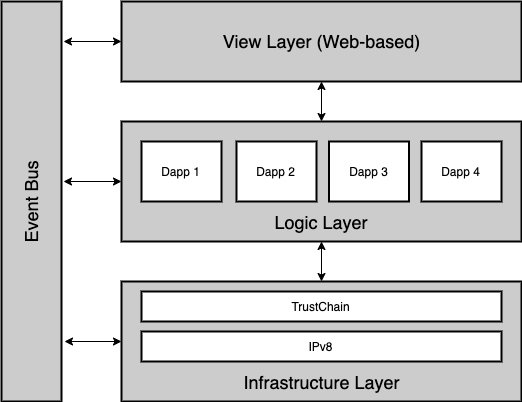
\includegraphics[width=0.5\textwidth]{images/architecture.png}
	\caption{\label{fig:architecture}}
\end{figure}

\section{Event-driven Architecture}

% event-driven architecture (event bus)

The framework is designed for running many different isolated applications. These applications consist out of separate modularized components that each run on different layers. Connecting these components together to form the application can quickly become a mess. To prevent this from happening, the framework makes use of an event-driven architecture. In such an architecture, actions are taken based on other actions happening in the system. Creating simple and maintainable logic. Input such as human interaction, network packets, creation of components, and/or system events, trigger corresponding actions in other parts of the system. An example of this would be the downloading of a module when a new one is discovered. This event system is located in the infrastructure layer and communicates with the other layers through the event bus. This event bus allows other parts of the system to hook on to specific events triggered by certain actions. To allow components to hook onto such an event they have to register an event handler with the event bus for the types of events it wants to act on.

\section{View Layer}

% view layer interface (events, rest endpoint)

The view layer contains the components that deal with human interaction. These components consist out of user interfaces created using web technologies. The decision for using web-based user interface was made because it is the current day standard for making cross-platform compatible GUIs and it allows for easy decoupling between itself and the logic behind it.

A view layer component consists out of a HTML, CSS, and javascript website. This website is run as a standalone component and connects to its logic counterpart through a REST API. This decouples the user interface part of the application and allows it to be interchanged. Multiple different GUIs could be offered for the same application.

When a new view component is added to the system, it needs to know how to connect to the logic component of the application. It does this by triggering an event on the event bus, specific for the type of application it belongs to, indicating it is requesting an endpoint address. The logic component is subscribed to this event. Its registered handler will return the REST API endpoint address back to the view component through the event bus.

To define a view component, a special file has to be created: view-component.json. This definition file stores the attributes and the settings of the view component. Attributes of the file include: name, version, app-tag (Application tag used for hooking on to the logic component). Each view component also needs to have a directory named public which contains the index.html file. An example structure can be found below.

\begin{itemize}
	\item view-component.json
	\item public \begin{itemize}
		\item index.html
		\item Other HTML/CSS/javascript resources
	\end{itemize}
\end{itemize}

% Component definition: component.json, properties, directory structure

\section{Logic Layer}

% logic layer (dapps, dapp interface, types of dapps, dapp definition language, versioning, states, live re-loading, caching strategies, identity profiles (anonymous, shared identities), isolation)

The logic layer contains the components that deal with the functionality of the application. Each component is defined by a file called: component.json located in the root of the component's directory. This file stores the properties and the settings of the logic component. The default properties that need to be defined are: name, version, app-tag, type. The component can be one of three types: Code, Overlay, or Service

\subsection{Code Component}

The code component consists out of a Python script without decentralized functionality that is executed on the host system. These types of components can be used as simple code scripts or as building blocks for bigger and more complex components. An example of this would be an updater script or an interface implementation.

In addition to the default properties a logic component defines, the code component also defines a function that needs to be executed when the module is run.

\subsection{Overlay Component}

The overlay component consists out of a decentralized overlay built on the IPv8 network. This component requires all files necessary to run an IPv8 overlay. This type of component runs in a shared environment and can have access to other overlay components in this same environment.

In addition to the default properties a logic component defines, the overlay component also defines the overlay class and overlay settings

% specific component properties

\subsection{Service Component}

The service component consists out of a twisted service. This service type can be used to run processes in the background or isolate certain processes from other processes in the system.

In addition to the default properties a logic component defines, the service component also defines the service class.

% specific component properties

\subsection{Versioning}

A system without versioning can quickly become infected and would make it difficult to track on which iteration the system is running. That is why each component has a component name and a version. The name property is a unique value for each component used to differentiate it from other components. The version property is value that is incremented every time a change has been made to the component. Together these properties form the identifier of the component.

\section{Infrastructure Layer}

infrastructure layer is responsible for providing network functionality and lower level functionality like storage. It accomplishes this through multiple different modules. Twisted is responsible for allowing pseudo multi threading through event-driven architecture. IPv8 is responsible for providing overlay functionality to run decentralized applications in and on the framework. TrustChain is responsible for providing a decentralized blockchain storage. LibTorrent is responsible for providing file transport services.

\section{Identity Profiles}

In peer-to-peer systems each peer in an overlay has to have an identity. This identity determines the trust and association within and across overlays. This identity can be shared between different overlays or each overlay can use its own identity. If two overlays use the same identity, one overlay can benefit from the built up trust and reputation of another overlay. However, actions performed by one overlay can also have a negative trust impact on the other overlay. To allow applications to choose between the having a shared identity, having its own identity, or having an pseudo-random identity,  the framework provides a configuration option in the component.json to select what kind of identity profile is preferred..  

\section{System Strategies}

Since the framework deals with untrusted executable user code, the framework provides several different strategies that the user can select from to protect their system against possible threats from running this code.

\subsection{Download and Retention Strategy}

The framework allows the user to configure and replace the download and retention strategy. This strategy is responsible for choosing which components get downloaded and how long they are kept on the system. For the distribution of components it is necessary to download packages that might not be used by the host system itself, but are solely for the intent of distributing. Some users might want to take a different approach to accomplish this. The framework addresses this by allowing parts of its code to be replaced by other components written by a third-part or by the user itself.

\subsection{Isolated Execution}

Since all distributed components have to be executed on the host system for them to function, it can pose a security risk by running untrusted user code. To minimize the risk that this poses, the framework allows components to be run inside of an isolated execution environment using Docker. When this method is used an execution environment is setup inside of the docker engine and the code will be mounted inside of this container. This container will then be able to run the code in isolation. This method, however, will prevent other applications running on the system from communication to it. It does allow the view layer to communicate with the isolated components since this makes use of network sockets.

% infrastructure layer (TrustChain, IPv8, DB, LibTorrent, caching) 
\chapter{\label{chap:implementation}Implementation}

This chapter discusses the implementation details of the system described in the previous chapter. The thesis work aimed to create a proof-of-concept implementation to demonstrate the proposed concepts. 

% - module discovery gossip
% - rating and voting
% - code screenshots
% - LoC + code coverage stats

\section{Overview}

% What is implemented from the framework
% Proof of Concept code
% Can be optimized

This work took a prototyping approach to get to a functioning prototype rapidly and improve from there. All major concepts that were discussed in Chapter 3 were implemented in the proof-of-concept code base. The code was developed alongside the research and served as an evaluation of the principles being worked on. 

As the main purpose of the implementation is a proof-of-concept, this codebase is not optimized for a production environment. Various different performance and quality optimizations can be done to improve the quality of the implemented product. Examples of these optimizations include:

\begin{itemize}
	\item Implement caching for module database
	\item Remove verbose validations found all over the code
	\item Making the implementation more crash-resistant
	\item Better integrate the torrent library by hooking into its event system for notifications 
	\item Improve the user-friendliness
\end{itemize}

The final codebase can be found publicly on GitHub \footnote{https://github.com/mitchellolsthoorn/ipv8-module-loader}. The readme for the project can be found in Figure~\ref{fig:project-readme}. The programming language that was used for the prototype is Python. Python was chosen because it allows for rapid development and has access to a large collection of existing libraries. Since Python is dynamically typed and allows a lot of flexibility when it comes to security, it also made it easier to implement the proposed concepts in this programming language. The codebase consists out of 5000+ lines of code.

During the development of the implementation, several improvements were made and contributed to the overlay library used. This overlay library was only available on GitHub and needed to be used through Git Submodules. By working with the developers of the library we made changes to the library that allowed it to be distributed through the Python Pip package manager. This allows the library to be more easily integrated and used by other developers. Another improvement that was made to the library was a problem discovered in the REpresentational State Transfer (REST) protocol used for communicating with the library backend. This bug made it impossible for HTTP clients that implemented CQRS security to communicate with the library. We proposed a new base endpoint for the REST service that implemented this security protocol that all other endpoints extend from. This rewritten REST service was eventually merged into the main code base of the library. The pull requests for these changes can be found on the library's GitHub repository \footnote{https://github.com/Tribler/py-ipv8/pulls?q=is\%3Apr+is\%3Aclosed+author\%3Amitchellolsthoorn}.

\begin{figure}[h!]
	\centering
	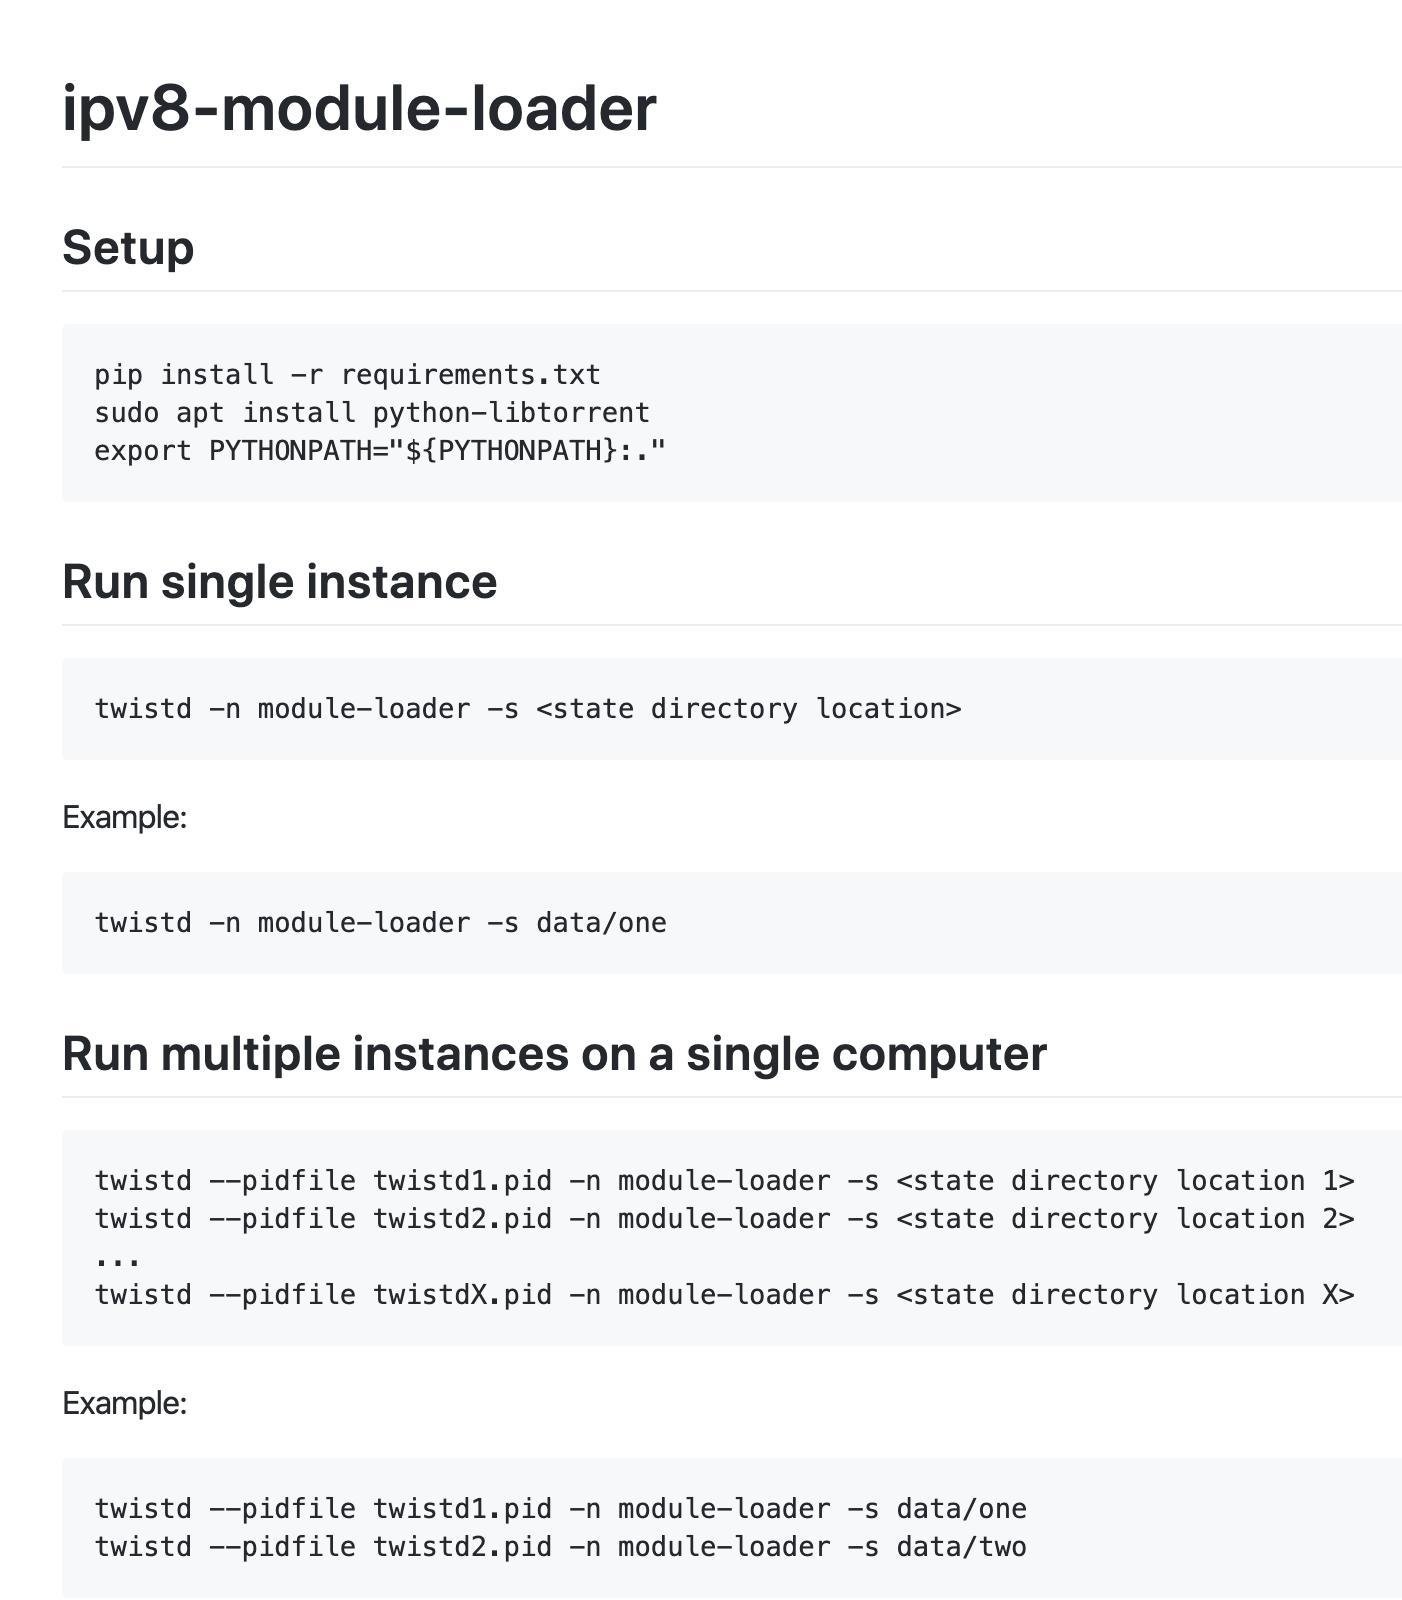
\includegraphics[width=0.8\textwidth]{images/readme.png}
	\caption{\label{fig:project-readme} Readme of the IPv8 module loader project.}
\end{figure}

\section{IPv8 - Overlay Library}

IPv8 is the underlying network overlay library used in the implementation. It is responsible for providing \textbf{authenticated} and \textbf{encrypted} communication between different peers (computer nodes) in the system. The framework abstracts the notion of physical addresses (IP addresses) in favor of public keys. This removes the need for applications that use this library to keep track of where different peers in the system are and how to move data between them. IPv8 simplifies the design of distributed overlay systems. 

Some other important aspects of the framework are its focus on:
\begin{itemize}
	\item \textbf{Privacy:} where it is possible to choose if messages should be identifiable to all peers in the network or only to the peers absolutely needed for the network connection (doesn't include the receiver). 
	\item \textbf{No infrastructure dependency:} allowing the network to function on its own run by the peers using the system. This is a very important aspect of the framework as it allows the framework to support itself, without needing external financing for server capacity.
	\item \textbf{NAT traversal:} making it possible to operate the network without static servers needed for overcoming the NAT issues that most peer-to-peer networks face.
	\item \textbf{Trust:} one of the most important aspects of peer-to-peer systems, as it is needed to mitigate free-riding issues in the network. In IPv8 trust is gained by recording a pattern of previous actions and storing these on a blockchain structure called TrustChain.
\end{itemize}

The last main aspect of the framework is \textbf{extensibility}. IPv8 makes use of a concept called overlays. Where a virtual network is created in the system related to one specific application domain or topic where different peers can subscribe to. This is a very powerful mechanism to allow extendability and modularization of an specific application. This makes it possible for user applications to be run alongside the FBase framework.

\section{Framework Structure}

This section will go over the major components of the code and explain the folder structure used in the implementation. The root directory of the project consists out of two folders:
\begin{itemize}
	\item \textbf{module\_loader:} The module loader directory serves as a python package for the entire code base of the prototype. All the major components of the framework are located in this directory.
	\item \textbf{twisted/plugins:} The twisted plugins directory is a mandatory location for the storage of the framework's main application files. This requirement comes from the library Twisted which IPv8 is built on. This library provides pseudo-multi-threading by implementing an event-based scheduler.
\end{itemize}

Inside the module loader python package, the following structure is used:

\begin{itemize}
	\item \textbf{CLI:} The CLI package contains all classes and logic related to the command-line user interface of the framework. This is the primary way to manage the network.
	\item \textbf{community:} The community package contains the overlay code. This includes the majority of all logic related to the FBase functionality.
	\item \textbf{event:} The event package contains all classes and functionality related to the main event bus of the FBase framework.
	\item \textbf{REST:} The REST package contains all REST endpoints needed to communicate with the FBase backend from other applications and services. This interface also allows user applications to communicate with their frontend
	\item \textbf{web:} The web directory contains the web frontend for the FBase framework. This is an alternative way of managing the framework next to the CLI.
\end{itemize}

\section{Community}

The community class is the main overlay class that manages all parts of the FBase module network. This class acts as the controller for all inputs and outputs of the system.

Figure~\ref{fig:community-code} shows snippets of the community code base as the central part of the application logic.

\begin{figure}[h!]
	\centering
	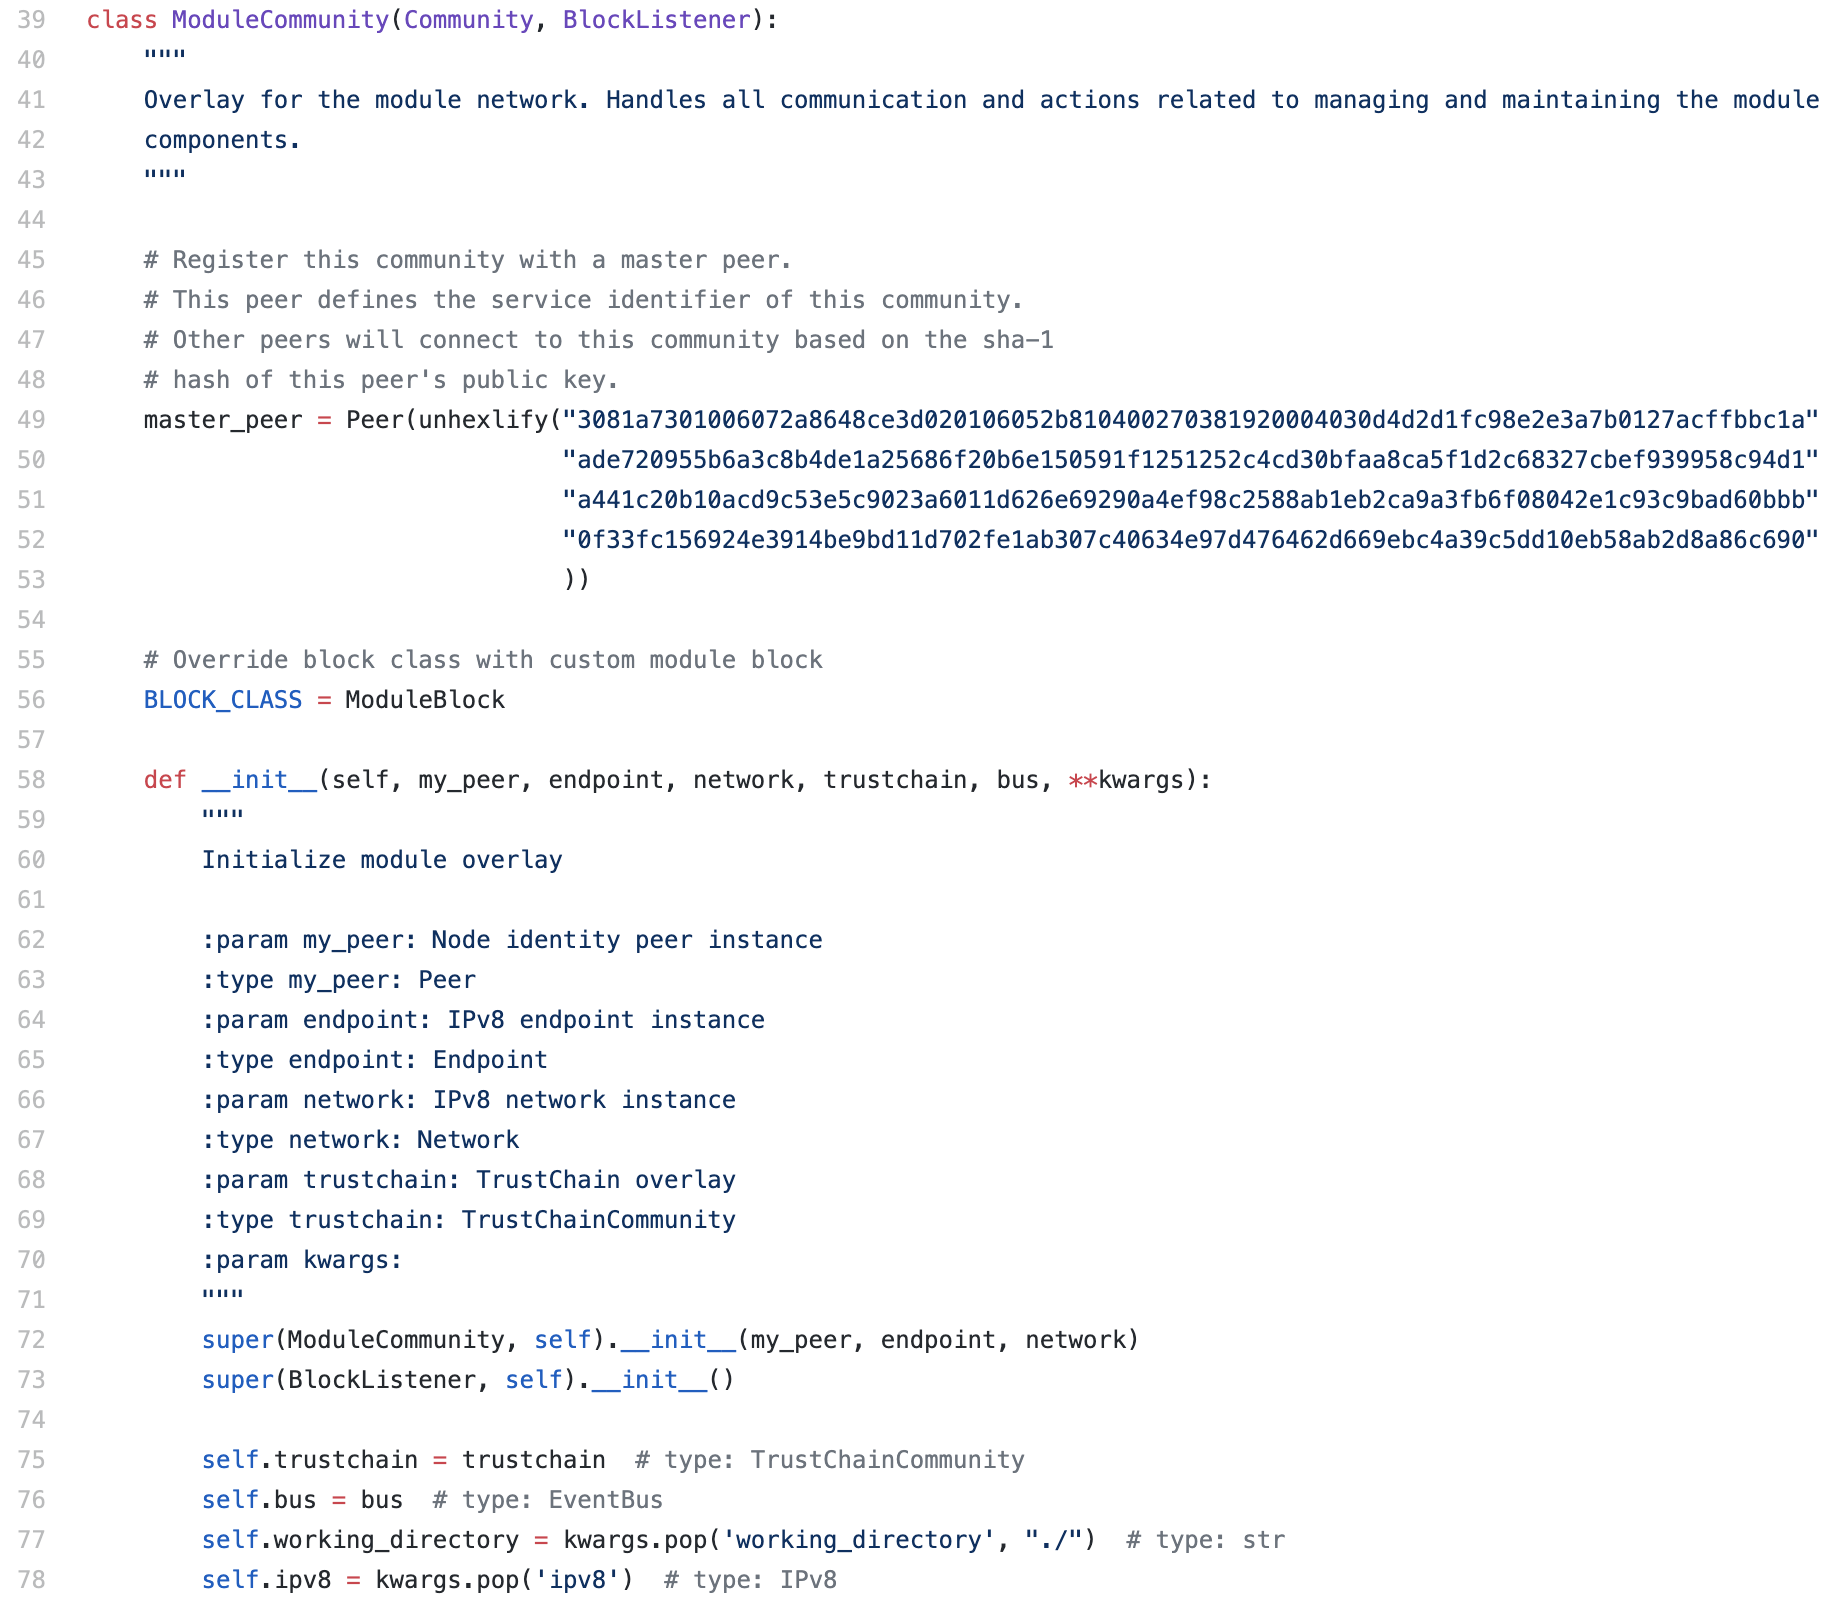
\includegraphics[width=\textwidth]{images/code-community-class.png}
	\caption{\label{fig:community-code}}
\end{figure}

\section{Event Bus}

The event bus that is implemented in the FBase prototype is built according to a PubSub design pattern. In this design pattern, modules can register themselves to receive messages when an event has been fired with a certain event type. These registered modules, also called subscribers, are stored in an array in memory. They only receive a call when that event is fired. Modules that publish events, called publishers, call the event bus with the message and the type of the message.

In the prototype, the event bus is implemented in code. For production use, however, it might be a good improvement to run the event bus as a separate process to speed up the performance when many events are being fired at a time. It would also allow multiple processes to be used to handle the actions performed by the subscribers. 

\section{Interface}

There are two interfaces through which the FBase framework can be managed. Originally only the CLI interface was used. Later in development, the web interface was added to allow the framework to be controlled from any platform the framework runs. This decision was made since the framework itself could be run cross-platform, but it could only be controlled from platforms that support a CLI.

\subsection{CLI}
The CLI interface operates through a command-line menu interface. This menu allows the user of the framework to run sets of actions. The general actions are

\begin{itemize}
	\item \textbf{List all modules:} This action provides a list with context actions. Each of these context actions is performed on the module that is selected by the user.
	\item \textbf{Create test module:} Create an empty test module that can be used for testing the distribution of modules through the network.
	\item \textbf{Create module:} Create a module from a module definition that exists on the file system. The module should already be created. This action only processes the module and prepares the metadata for publishing it on the network.
\end{itemize}

The context menu for each module shows information about the module. It includes the name of the module, the description, the identifier and the number of votes in the network for the module. Next to this information, there are also context actions that are displayed and can be called. The context actions include:

\begin{itemize}
	\item \textbf{Vote:} This context actions instructs the backend of the framework to sign the corresponding vote block that will be created. This vote block will then be distributed through the network.
	\item \textbf{Download:} The download context action retrieves the identifier of the module and starts the download of the module through the transport engine.
	\item \textbf{Run:} The run context action loads the module package namespace into the Python path of the framework. Afterward, it starts the application based on the instructions provided in the module.
\end{itemize}

Figure~\ref{fig:cli-interface} shows a screenshot of the CLI interface showing the list of discovered modules.

\begin{figure}[h!]
	\centering
	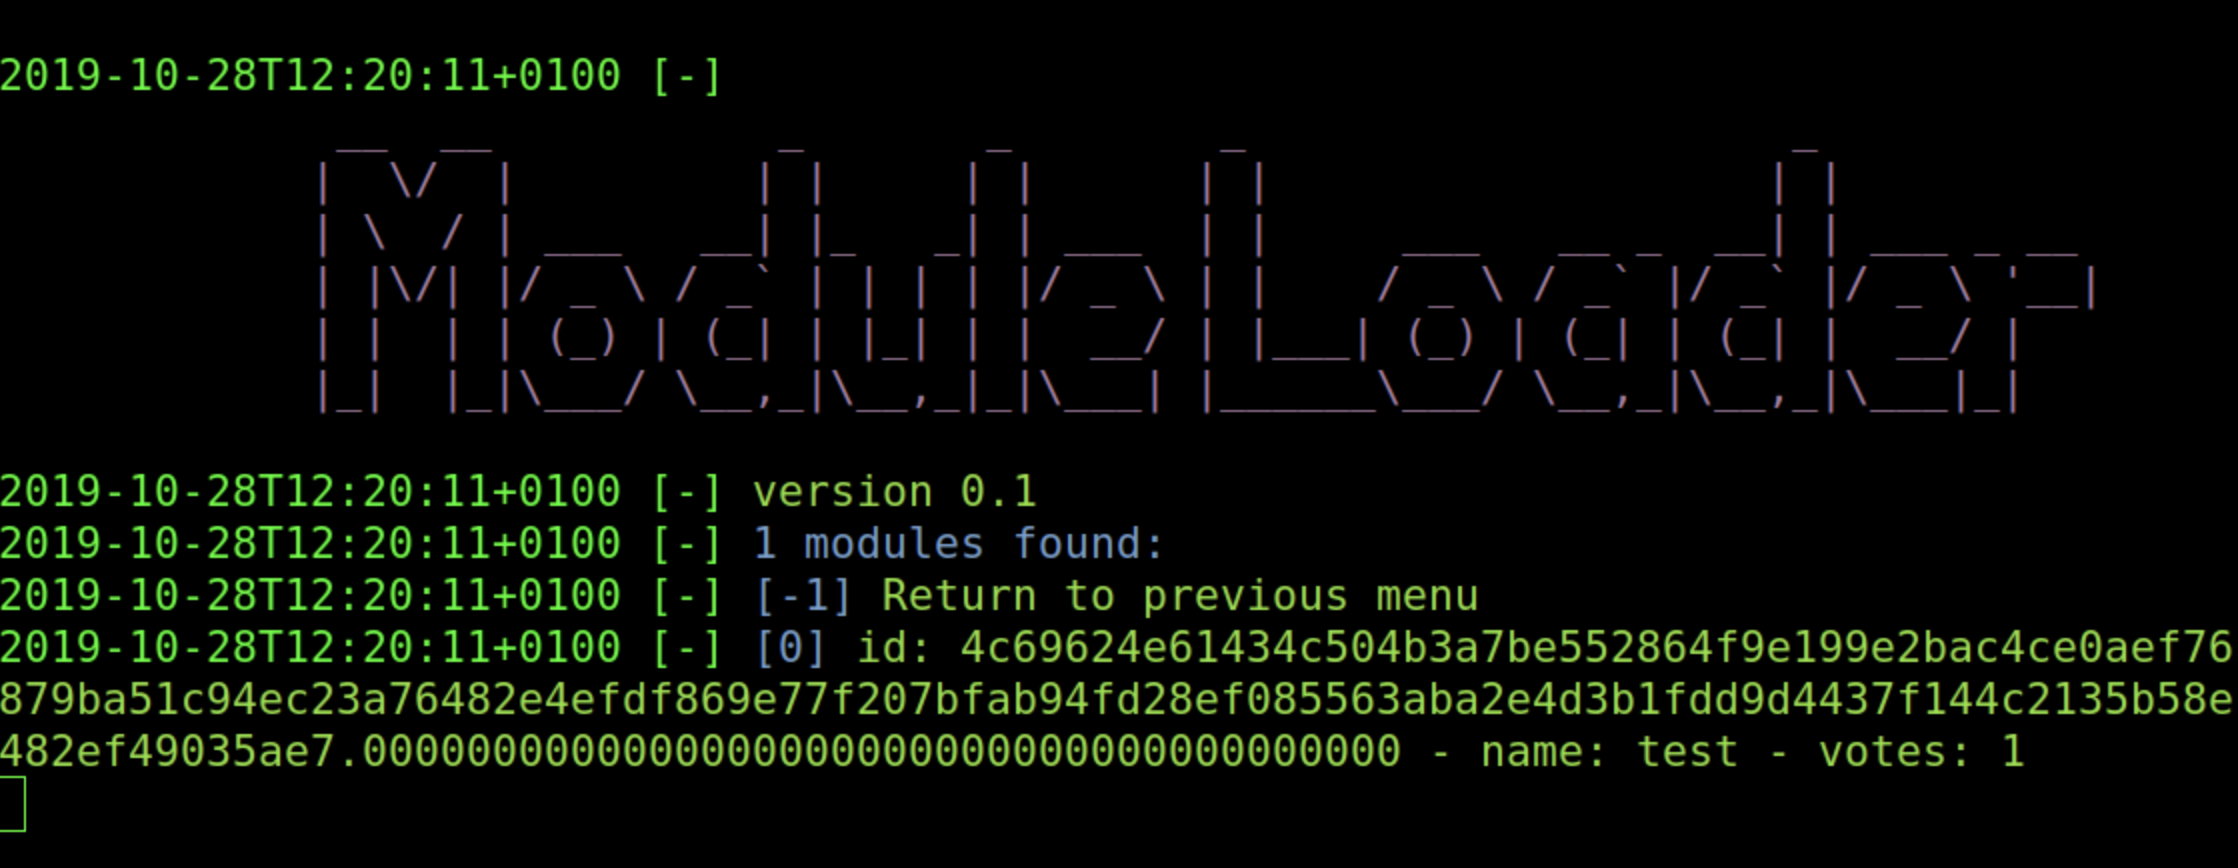
\includegraphics[width=\textwidth]{images/cli-interface.png}
	\caption{\label{fig:cli-interface} CLI interface of the FBase framework proof-of-concept.}
\end{figure}

\subsection{Web Interface}

The web interface is a website built with HTML, CSS, and JavaScript that runs as a standalone service that communicates with the FBase backend through the REST API. This interface allows to view all discovered modules, download them and run them. This interface does not allow a module to be created.

\section{REST Endpoints}

The FBase framework provides several REST endpoints on its API for the web interface to operate. These API endpoints can also be used by other applications to perform actions on the overlay network.

\begin{itemize}
	\item \textbf{Catalog:} The catalog endpoint is responsible for all actions related to the discovered modules on the network. This endpoint is mostly used for retrieving information about the modules available.
	\item \textbf{Downloads:} The downloads endpoint is responsible for managing modules that need to be downloaded or are already downloaded. Its actions include the downloading of modules, the deletion of modules from the host, and to retrieve the status of the downloaded modules.
	\item \textbf{Library:} The library endpoint is used to manage all modules that are currently being used by user applications on the framework.
	\item \textbf{Run:} The run endpoint provides actions to load and run the module that is specified.
	\item \textbf{Votes:} The votes endpoint is responsible for all actions related to voting and managing votes that have been performed.
\end{itemize}

\section{Module Structure}

This section will expand on the structure used for modules in the framework. Each module in the framework has to be a valid Python package. This is done to make it easier to import the module on runtime. This requires the module to have an \_\_init\_\_.py file in its root directory. Besides this, each module must also have a manifest.json file. This manifest file specifies the type of module and its information. Without this file, the module will not be detected and can not be run.

This manifest file contains a JSON dictionary. This dictionary contains key-value pairs for all the information required.

\begin{itemize}
	\item \textbf{Name:} Specifies the name of the module used for displaying in the user interface
	\item \textbf{Description:} Specifies the description of the module used for determining if a user wants to download and use the module 
	\item \textbf{Version:} Specifies the version of the module to determine if this is the most current version of the module
	\item \textbf{Type:} Specifies the type of the module, determining how it needs to be run and what kind of modules can require it.
	\item \textbf{Dependencies:} Specifies the other modules this module relies on.
\end{itemize}


\section{Module Distribution}
The module distribution method was chosen based on the ability to set up an integrated content distribution network that would work efficiently and scale. Since this is not the first time this is done and there already exist excellent solutions out there that could accomplish this.

\subsubsection{\textbf{Web protocols}}

Web protocols like HyperText Transfer Protocol (HTTP) and its secure variant HTTPS are a very common transfer protocol in the current day internet. It is used by all major Linux distribution to distribute the system packages, by websites for downloading content and watching videos. This protocol supports file transfer resumes, encryption. It, however, doesn't scale well when the same content has to be uploaded to multiple users and doesn't natively provide content verification.

\subsubsection{\textbf{BitTorrent}}

BitTorrent is the protocol used by all BitTorrent clients. It provides encryption, content verification, file transfer resumes, and scales efficiently when large amounts of the same content have to be distributed thanks to its mesh architecture. That is why this protocol was selected as the basis of the module distribution of this work.

BitTorrent also has the advantage of having a Distributed Hash Table (DHT). This DHT stores all information about who has a copy of the content and the metadata needed to download it in a distributed fashion. This removes the need for FBase to implement its own mechanism for this.

BitTorrent is the protocol used in the proof-of-concept.

\section{Discovery and Voting}

When a suitable transfer protocol is chosen, the next step was to make it possible for modules to be discoverable by all nodes in the system. Since we were already building our framework on top of the IPv8 peer-to-peer communication library. We decided it would be a good fit to use this to accomplish our goal since it was very suited for bulk small size data gossiping. So this became our chosen method of module discovery.

Since IPv8 also provides a block-chain storage back-end it was an perfect opportunity to also implement voting on the IPv8 library.

When a vote is done a block is created to represent this vote. This block is then stored on a blockchain. The reason we store the votes on the blockchain is to make votes irrefutable. Voting is unidirectional. Permission should not be needed from the other side. This is represented in the blockchain by only one party signing the vote. Storing votes on the blockchain also prevents malicious use of votes to promote one's module.

\section{Blockchain}

The FBase prototype is built on the TrustChain ledger introduced by Otte et al. We identified two advantages of TrustChain over other pairwise distributed ledgers like R3 Corda and Nano. 

First, TrustChain focuses on fraud detection instead of prevention and as a result, does not require network-wide consensus. This makes TrustChain a lightweight and simple data structure.

Second, TrustChain is already used as transaction fabric within a self-sovereign, decentralized identity system, described in the work of Stokkink et al. Availability of a self-sovereign identity system aligns with our requirement for strong, long-lived identities.
\chapter{\label{chap:evaluation}Evaluation}

% - trust explorer example
% - 9 fully functional modules
% - demonstrate the viability of run-time changes and alternative algorithmic approaches
% - open questions:
%   - how do we evaluate this?
%   - how do we show that it works as intended?
%   - we successfully bypassed the Android security model with protection against dynamic code injection using Webview
%   - pure technical (module loading times, memory usage impact, event-driven impact, event processing workload analysis, peak performance estimation)
%   - Github/NodeJS/Debian replacement workload analysis ("github is the largest code host in the world, with 20 million users and more than 57 million repositories"

This chapter will evaluate the proposed framework, FBase, described in Section~\ref{chap:design}. The evaluation consists of two parts, which will show if FBase, satisfies the requirements determined in Chapter~\ref{chap:requirements}:\newline

\begin{itemize}[nosep]
	\item Testing if the concept works and is viable.
	\item Examining the effectiveness of the discovery protocol% and the module communication.
\end{itemize}

\section{Testing the Viability of the Concept}

To determine if the concept works and is viable, this thesis uses one non-trivial use-case. This use-case comes from a project called Tribler.

\subsection{Tribler}

Tribler is an open-source community-driven decentralized BitTorrent client being developed and researched at the Delft University of Technology. Its main feature is that it allows anonymous peer-to-peer communication by default. It is built on the underlying network library IPv8, also being worked on by the same group.

Besides handling the tasks of a standard BitTorrent client, Tribler also makes it possible to:

\begin{itemize}
	\item \textbf{Search for content: } allowing the program to operate independently of external content search providers that could be blocked and made it immune to limiting external actions such as legal constraints. Which is happening more frequently nowadays.
	\item \textbf{Torrent anonymously: } routing torrent traffic through anonymized tunnels that operate using the same principle as the TOR stack. Providing pseudo-anonymity for the two end and other observing parties.
	\item \textbf{Accumulate trust: } all torrenting metadata is stored in a way that is not linked to an physical identity or an IP address. This data is then translated into a trust score by calculating the ratio between the amount of traffic communicated across the network. A positive seed ratio (the ratio between uploading content and downloading content) indicated a positive trust value.
	\item \textbf{Trade trust: } With this trust system it is possible to prioritize or refuse services for particular users. To increase the incentive for having a large seeder network and therefore a high trust value, Tribler allows users with a large amount of uploaded content to exchange this gathered trust for currency on the built-in marketplace inside the Tribler application.
\end{itemize}

This trust value, expressed as reputation inside the Tribler application, can be described as an up- and download currency in a reputation-based peer-to-peer network. When a peer uploads more than it downloads, the reputation of that peer increases, and the peer can download more effectively.

\subsection{Trust Experiment}

The experiment consists of conducting a use-case study, by creating a fully functioning example that demonstrates the composition and construction of an application with interchangeable trust models. This application will consist of 6 components:

\vspace{0.5cm}

\begin{minipage}[c]{0.45\textwidth}
	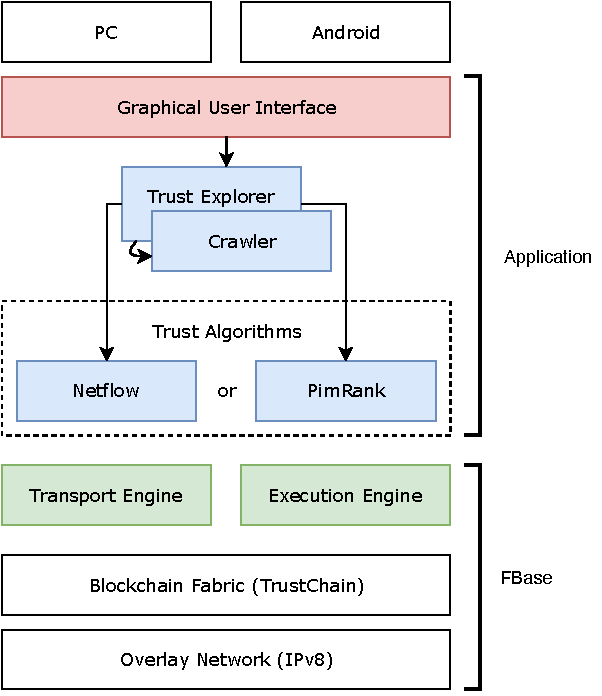
\includegraphics[width=\textwidth]{images/evaluation-trust-experiment-overview2.pdf}
\end{minipage}
\hfill
\begin{minipage}[c]{0.45\textwidth}
	{\large\textbf{Componenets:}}
	\begin{itemize}
		\item Test Application GUI (view layer)
		\item Trust Explorer (logic layer)
		\item Trust Crawler (logic layer)
		\item Trust Algorithm 1 (logic layer)
		\item Trust Algorithm 2 (logic layer)
		\item Execution Engine (infrastructure layer)
		\item Transport Engine (infrastructure layer)
	\end{itemize}
\end{minipage}

\vspace{0.5cm}

%Figure~\ref{fig:experiment} shows an overview of the example application.
The domain of trust was chosen since this is a very interesting use-case that has not been explored yet in other works. It allows users of a system to define their own notion of the concept of trust and apply this to their system without requiring extensive knowledge about each application they are using. For this experiment, this work makes use of two different trust algorithms: Netflow and PimRank. These two algorithms act as an example for this experiment.

%\begin{figure}[h]
%	\centering
%	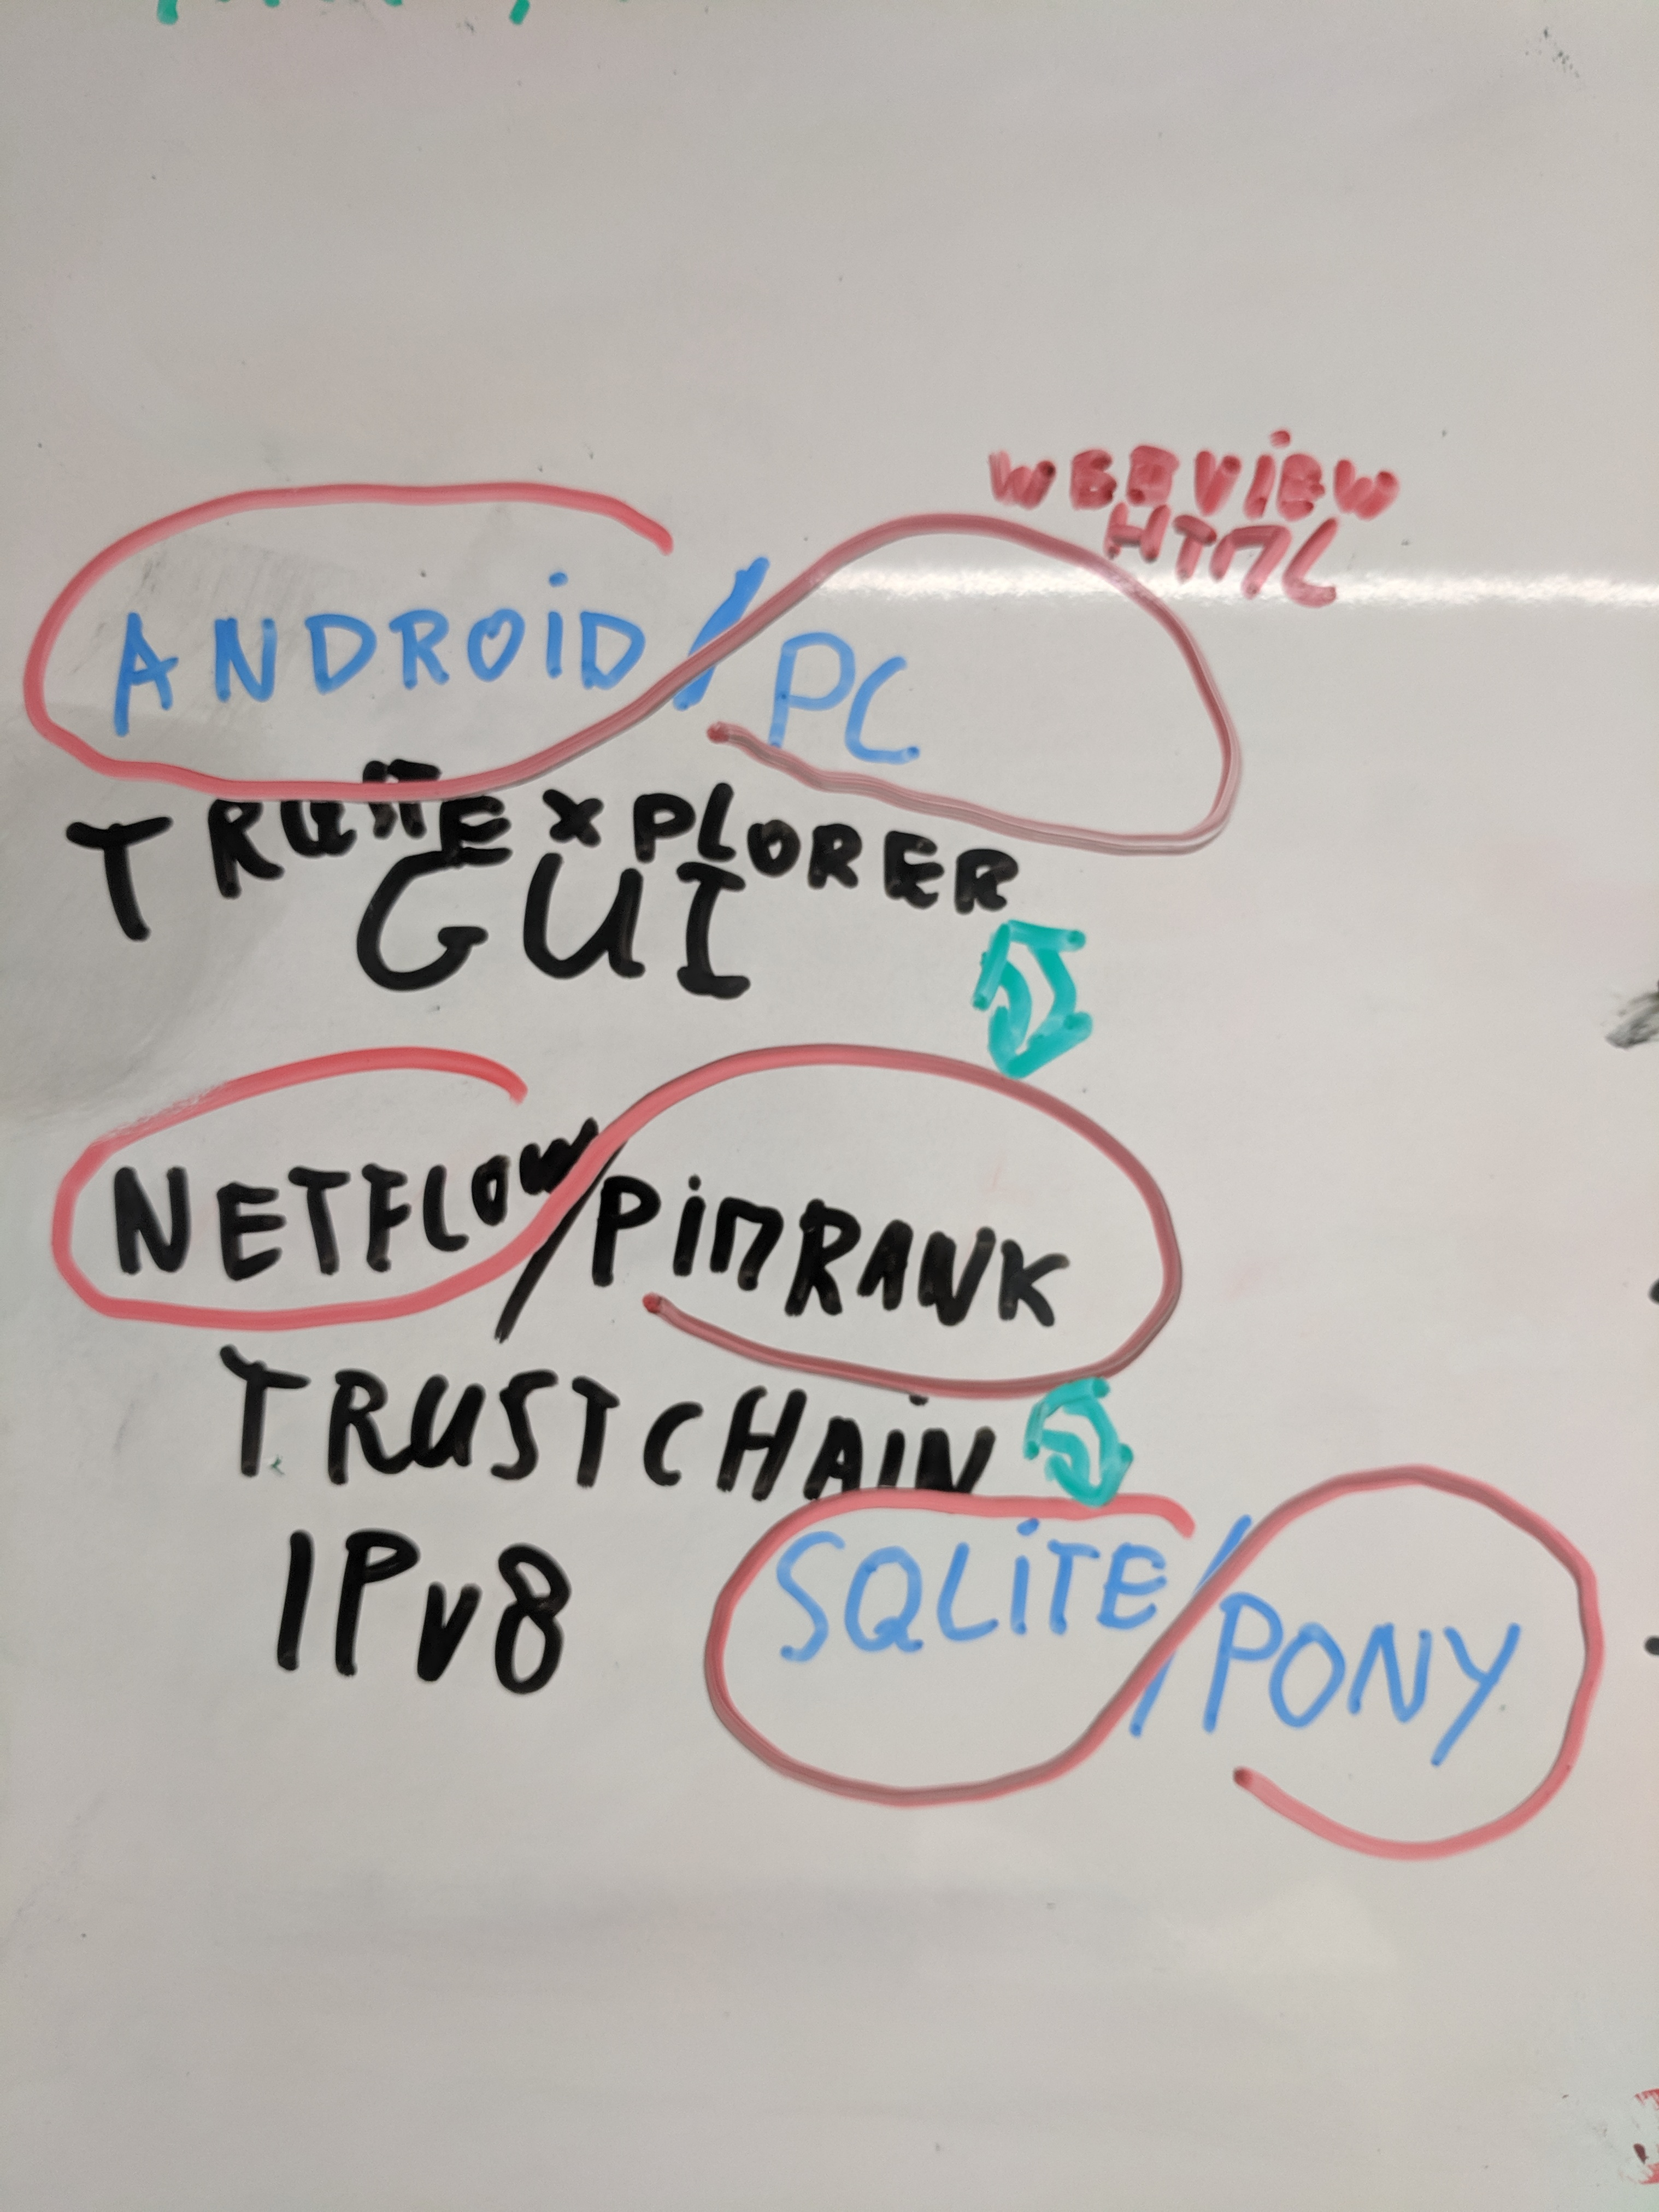
\includegraphics[width=0.5\textwidth]{images/experiment.jpg}
%	\caption{\label{fig:experiment} Trust experiment use-case}
%\end{figure}

\subsubsection{\textbf{Trustworthiness Experiment (5 stars vs 25 starts)}}

To test the viability of the framework has a whole and its concept of discovery through social trust, this work has performed a trustworthiness experiment to test if the proposed concept is viable for the purpose it is created for.

In this experiment the speed of modules that are distributed through the network are measured through the number of steps it has to make in the discovery algorithm. The experiment was run with a case of 5 stars and a case of 25 stars. The starts of an author represent the trustworthiness. This will influence if other nodes in the network vote on the module.

\begin{figure}[h]
	\centering
	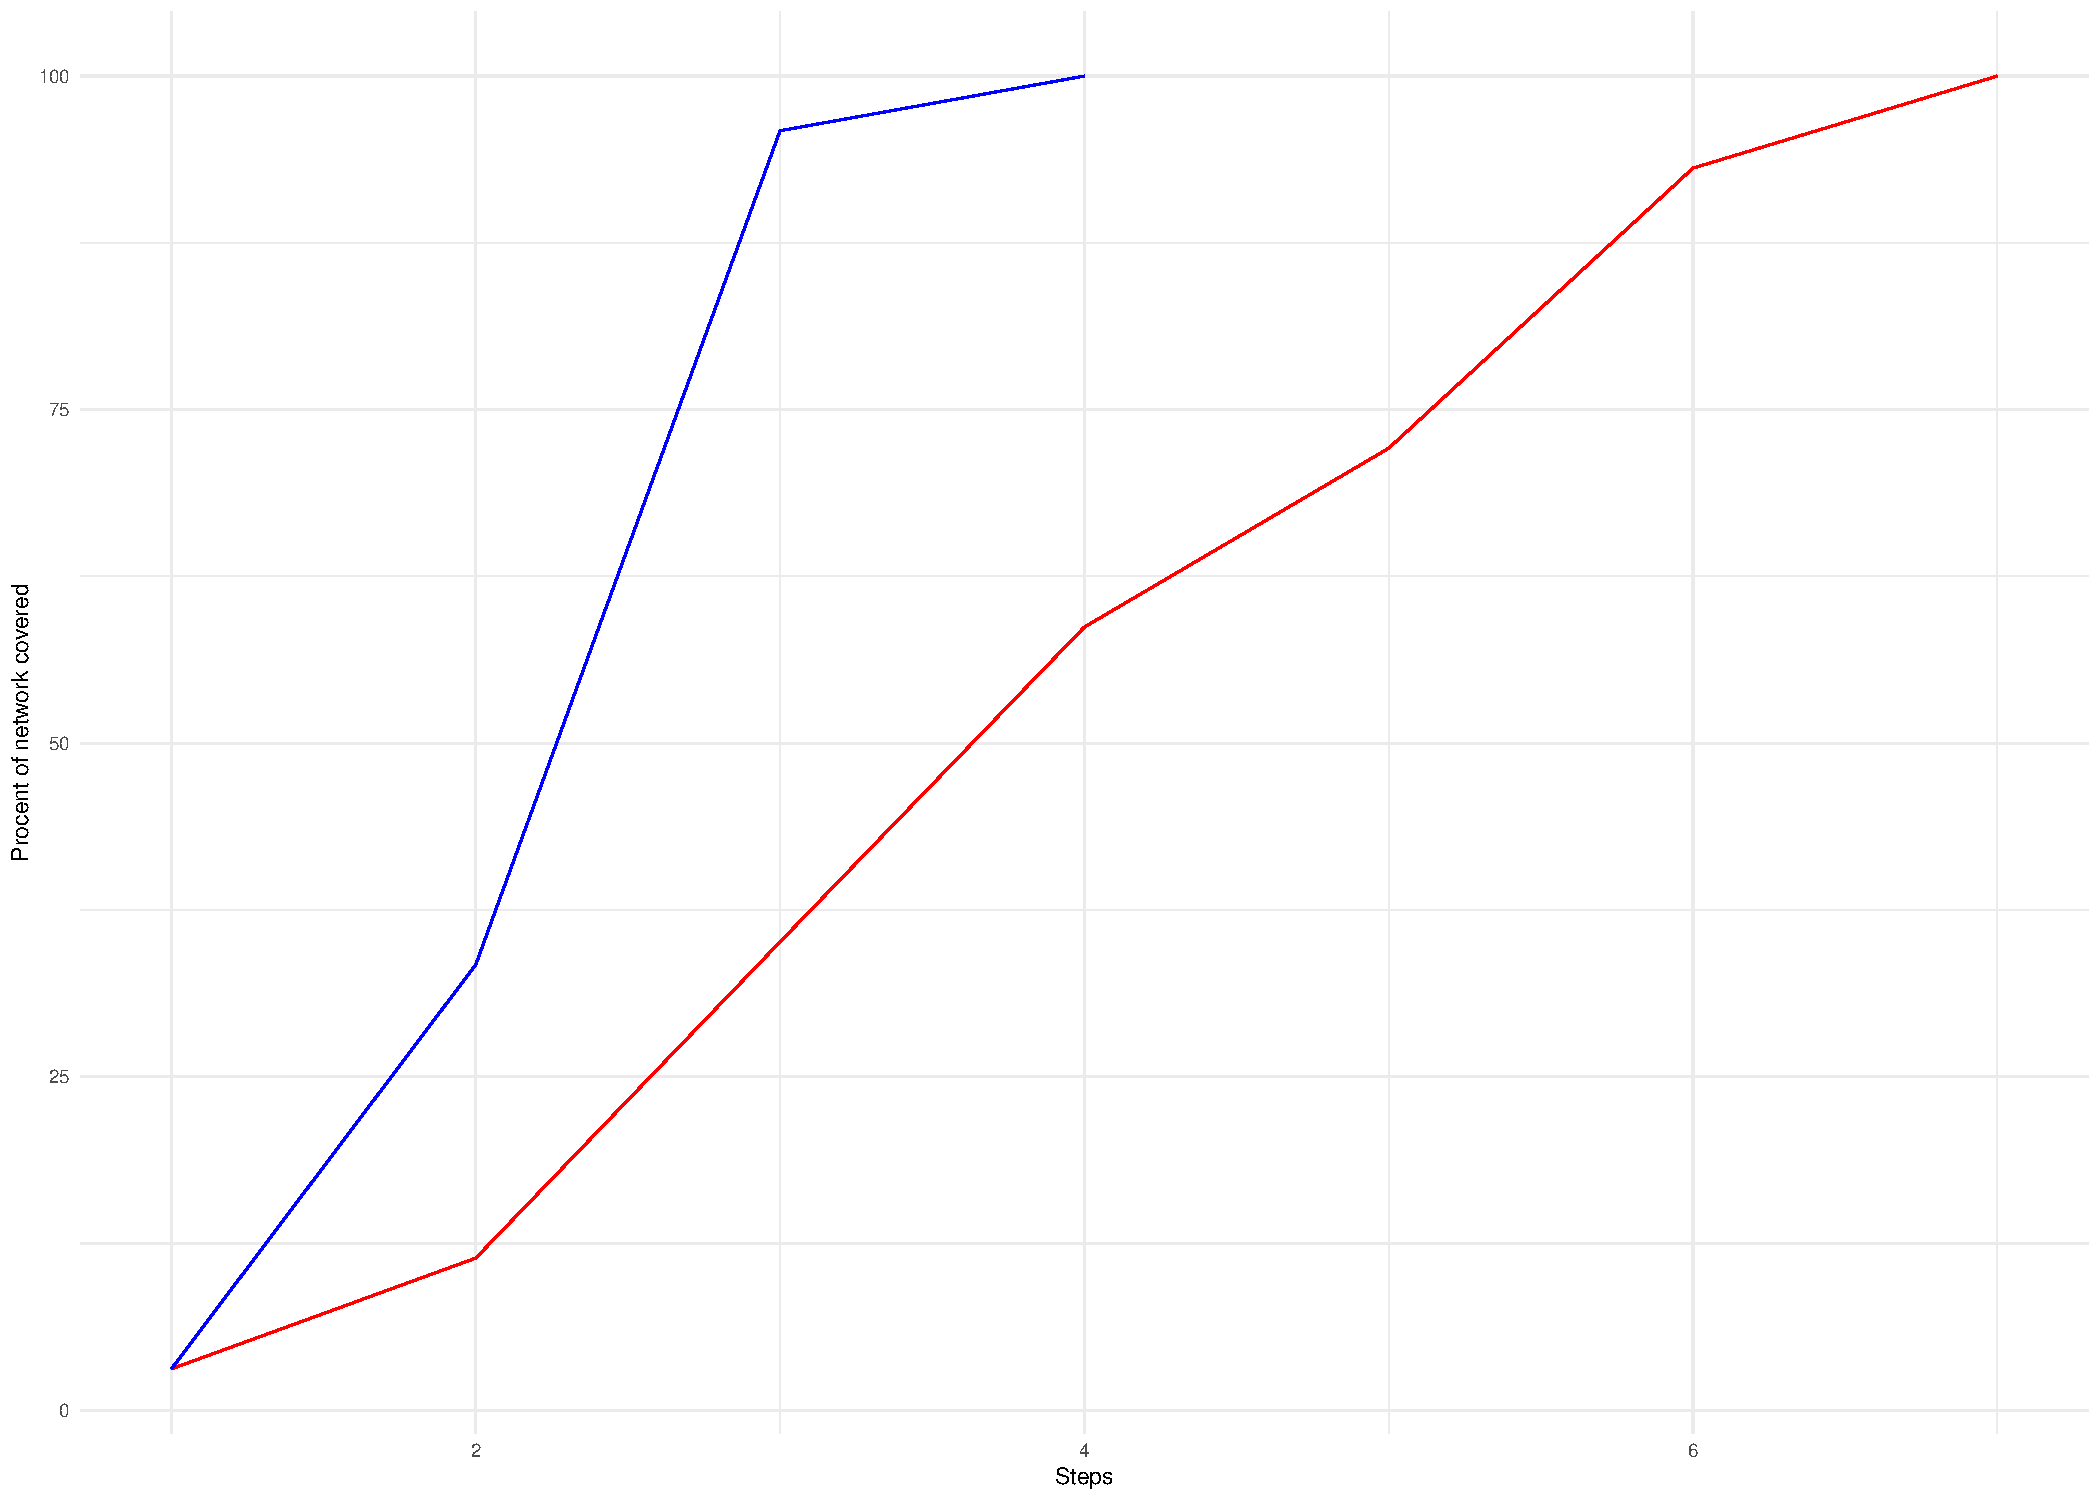
\includegraphics[width=0.8\textwidth]{images/trust.pdf}
	\caption{\label{fig:balance-scale} Trust experiment between 5 starts (red) and 25 stars (blue) authors.}
\end{figure}

\subsubsection{\textbf{CPU and Memory Breakdown}}

To test if the framework is efficient enough to operate applications running on top of it. This work has performed an experiment to see what the resource usage is of the framework under different scenarios.

\begin{figure}[h]
	\centering
	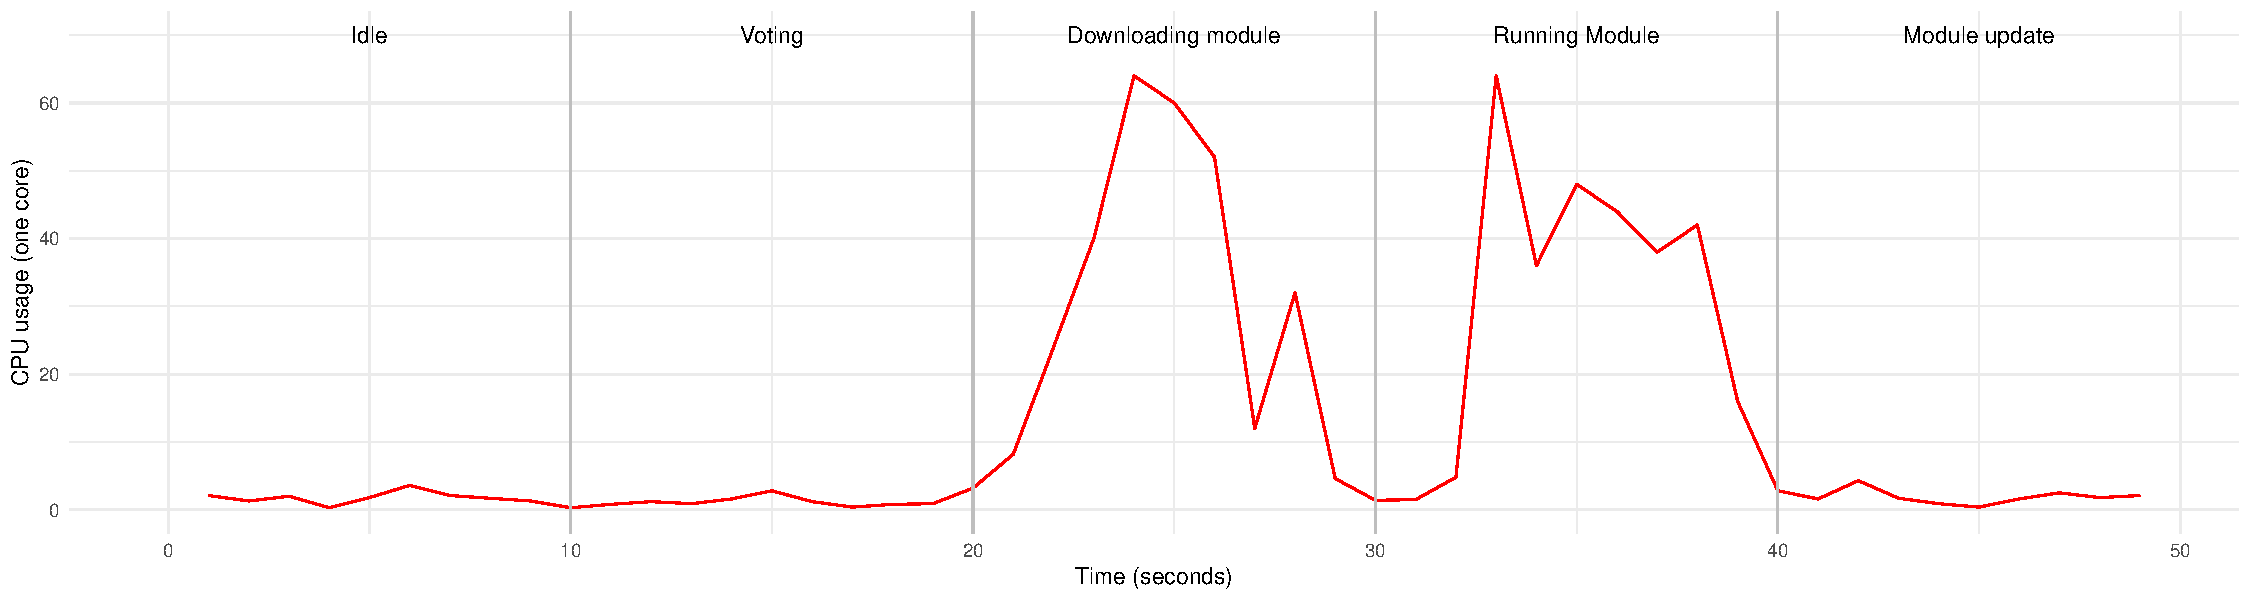
\includegraphics[width=1\textwidth]{images/cpu.pdf}
	\caption{\label{fig:balance-scale} CPU usage of FBase.}
\end{figure}
\begin{figure}[h]
	\centering
	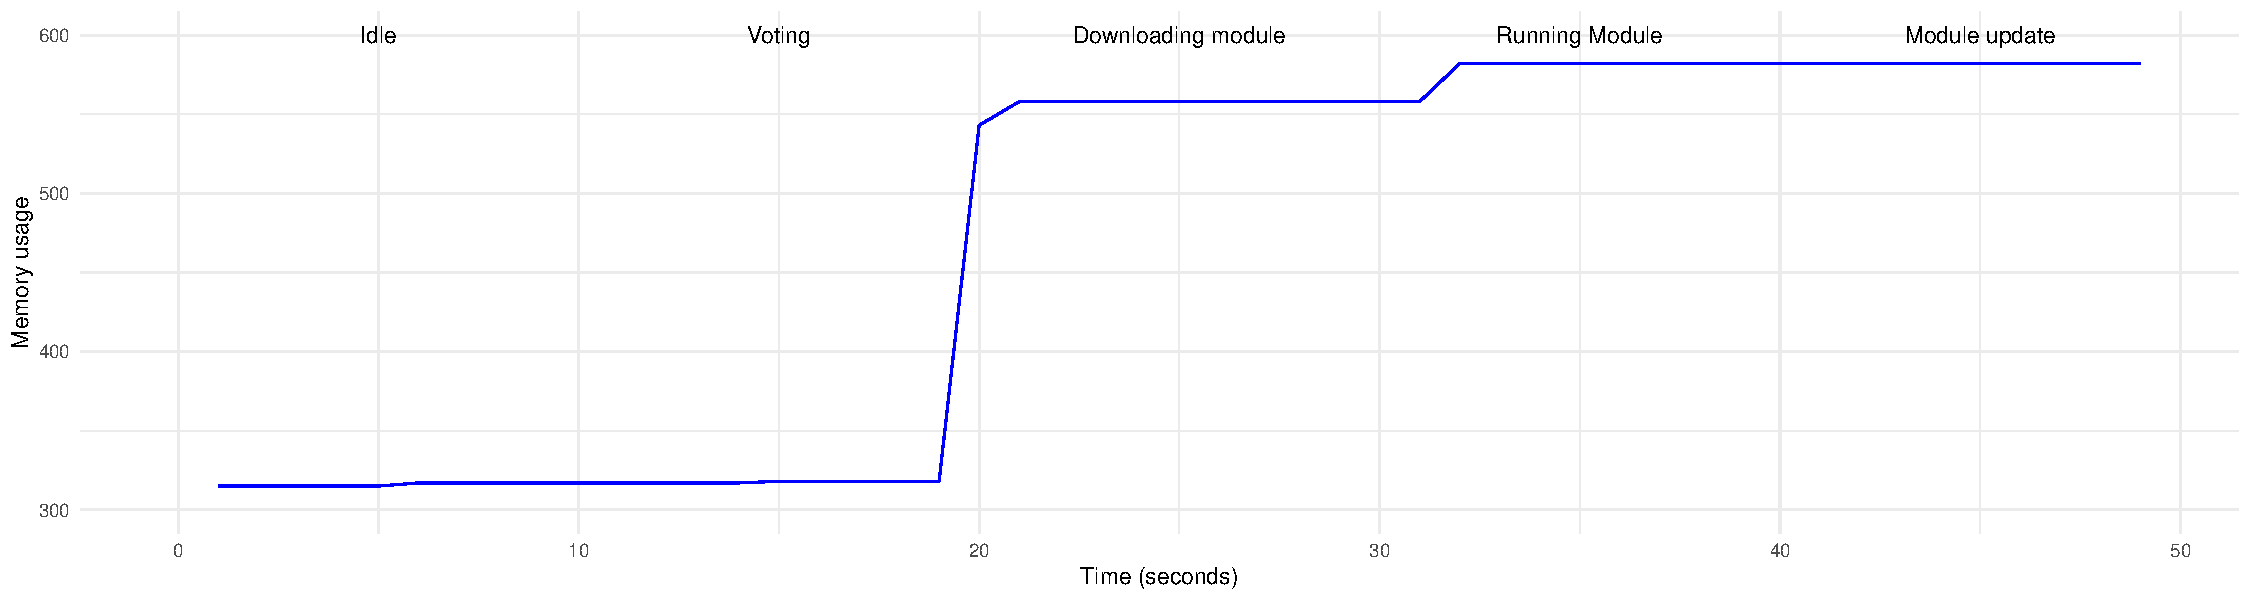
\includegraphics[width=1\textwidth]{images/mem.pdf}
	\caption{\label{fig:balance-scale} Memory usage of FBase.}
\end{figure}

\subsection{Mobile App Experiment}

To test the robustness and flexibility of the framework, an experiment was performed to try to create a proof-of-concept prototype of an Android application that could run the same stack of code to extend the ecosystem to mobile platforms. Since the two major mobile platforms (Android, iOS) only run applications custom made for these platforms, different methods had to be explored. Because iOS has a very restricted development environment and strict security policies, this route was not further explored.

The Android platform allows app developers to run Java, Kotlin (Java-based), and C. The desired framework language (Python) does not natively run on this platform. Converting the project code and dependencies is not a simple or maintainable method. This approach, however, also would not work. To improve security, the Android platform makes use of app scanning to verify that the executables haven't been tampered with. This security method severely hinders the working of the framework, since more functionality is added by the distribution of applications through its peer-to-peer network. These new code inclusions would trigger warnings in the Android security system and would block the app.

To circumvent this, a un-official method was used to package all the necessary code, dependencies, and executables as a single file and execute this as a C service on the Android platform. To accomplish this, a project called Python-for-Android was used. Python-for-Android is a build script that compiles the desired Python system version and Python dependencies for the ARM platform and creates a directory structure that can be used to run on Android. In Figure~\ref{fig:android-architecture} and overview of the Android app structure can be seen.

\begin{figure}[ht!]
	\centering
	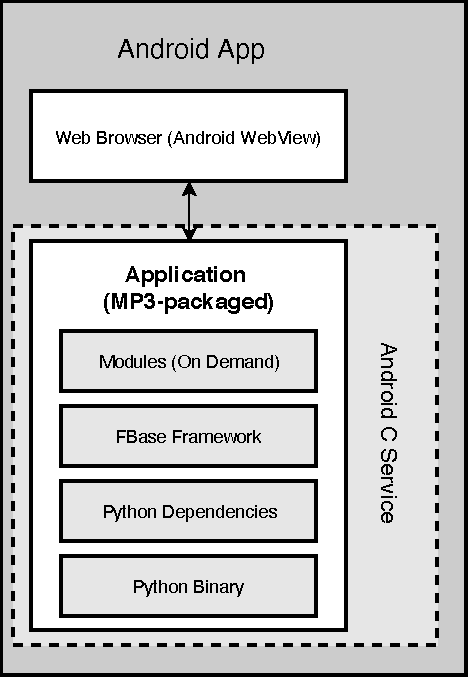
\includegraphics[width=0.5\textwidth]{images/evaluation-android-app.pdf}
	\caption{\label{fig:android-architecture} Android app architecture.}
\end{figure}

Since the Android app is needed to interact with the C service in the background, a part of the app had to be written in either Java or Kotlin. To keep this amount of code to a minimum, a decision was made to create all GUIs in web technologies, so the view layer can be shared between mobile and desktop platforms. This decision made it possible to include a web browser as the only component written for the mobile platform. This web browser can then interact with the webserver and REST API running on the C service.

To package the executable code in a way that would not trigger the Android security system, the code had to be bundled in a single file, disguised as an MP3. This format does not get checked by the Android security system and therefore can be used for this work. Underneath the extension, the code is packaged as a GZIP Tar-archive. Upon running the Android application, this MP3 file is unpacked in the application space of the app and the C service is started with the right configuration to run the code.

%In Figure~\ref{fig:android-app} a screenshot can be seen of the framework running with a test dApp on the Android platform. 

Development was stopped after reaching the proof-of-concept stage as it is not the main goal of this work and the development cycle is very tedious and slow. Each time a change or addition is made to the Framework the entire app structure has to be rebuild. This process can take up to 20 minutes. 

%\begin{figure}[h!]
%    \centering
%    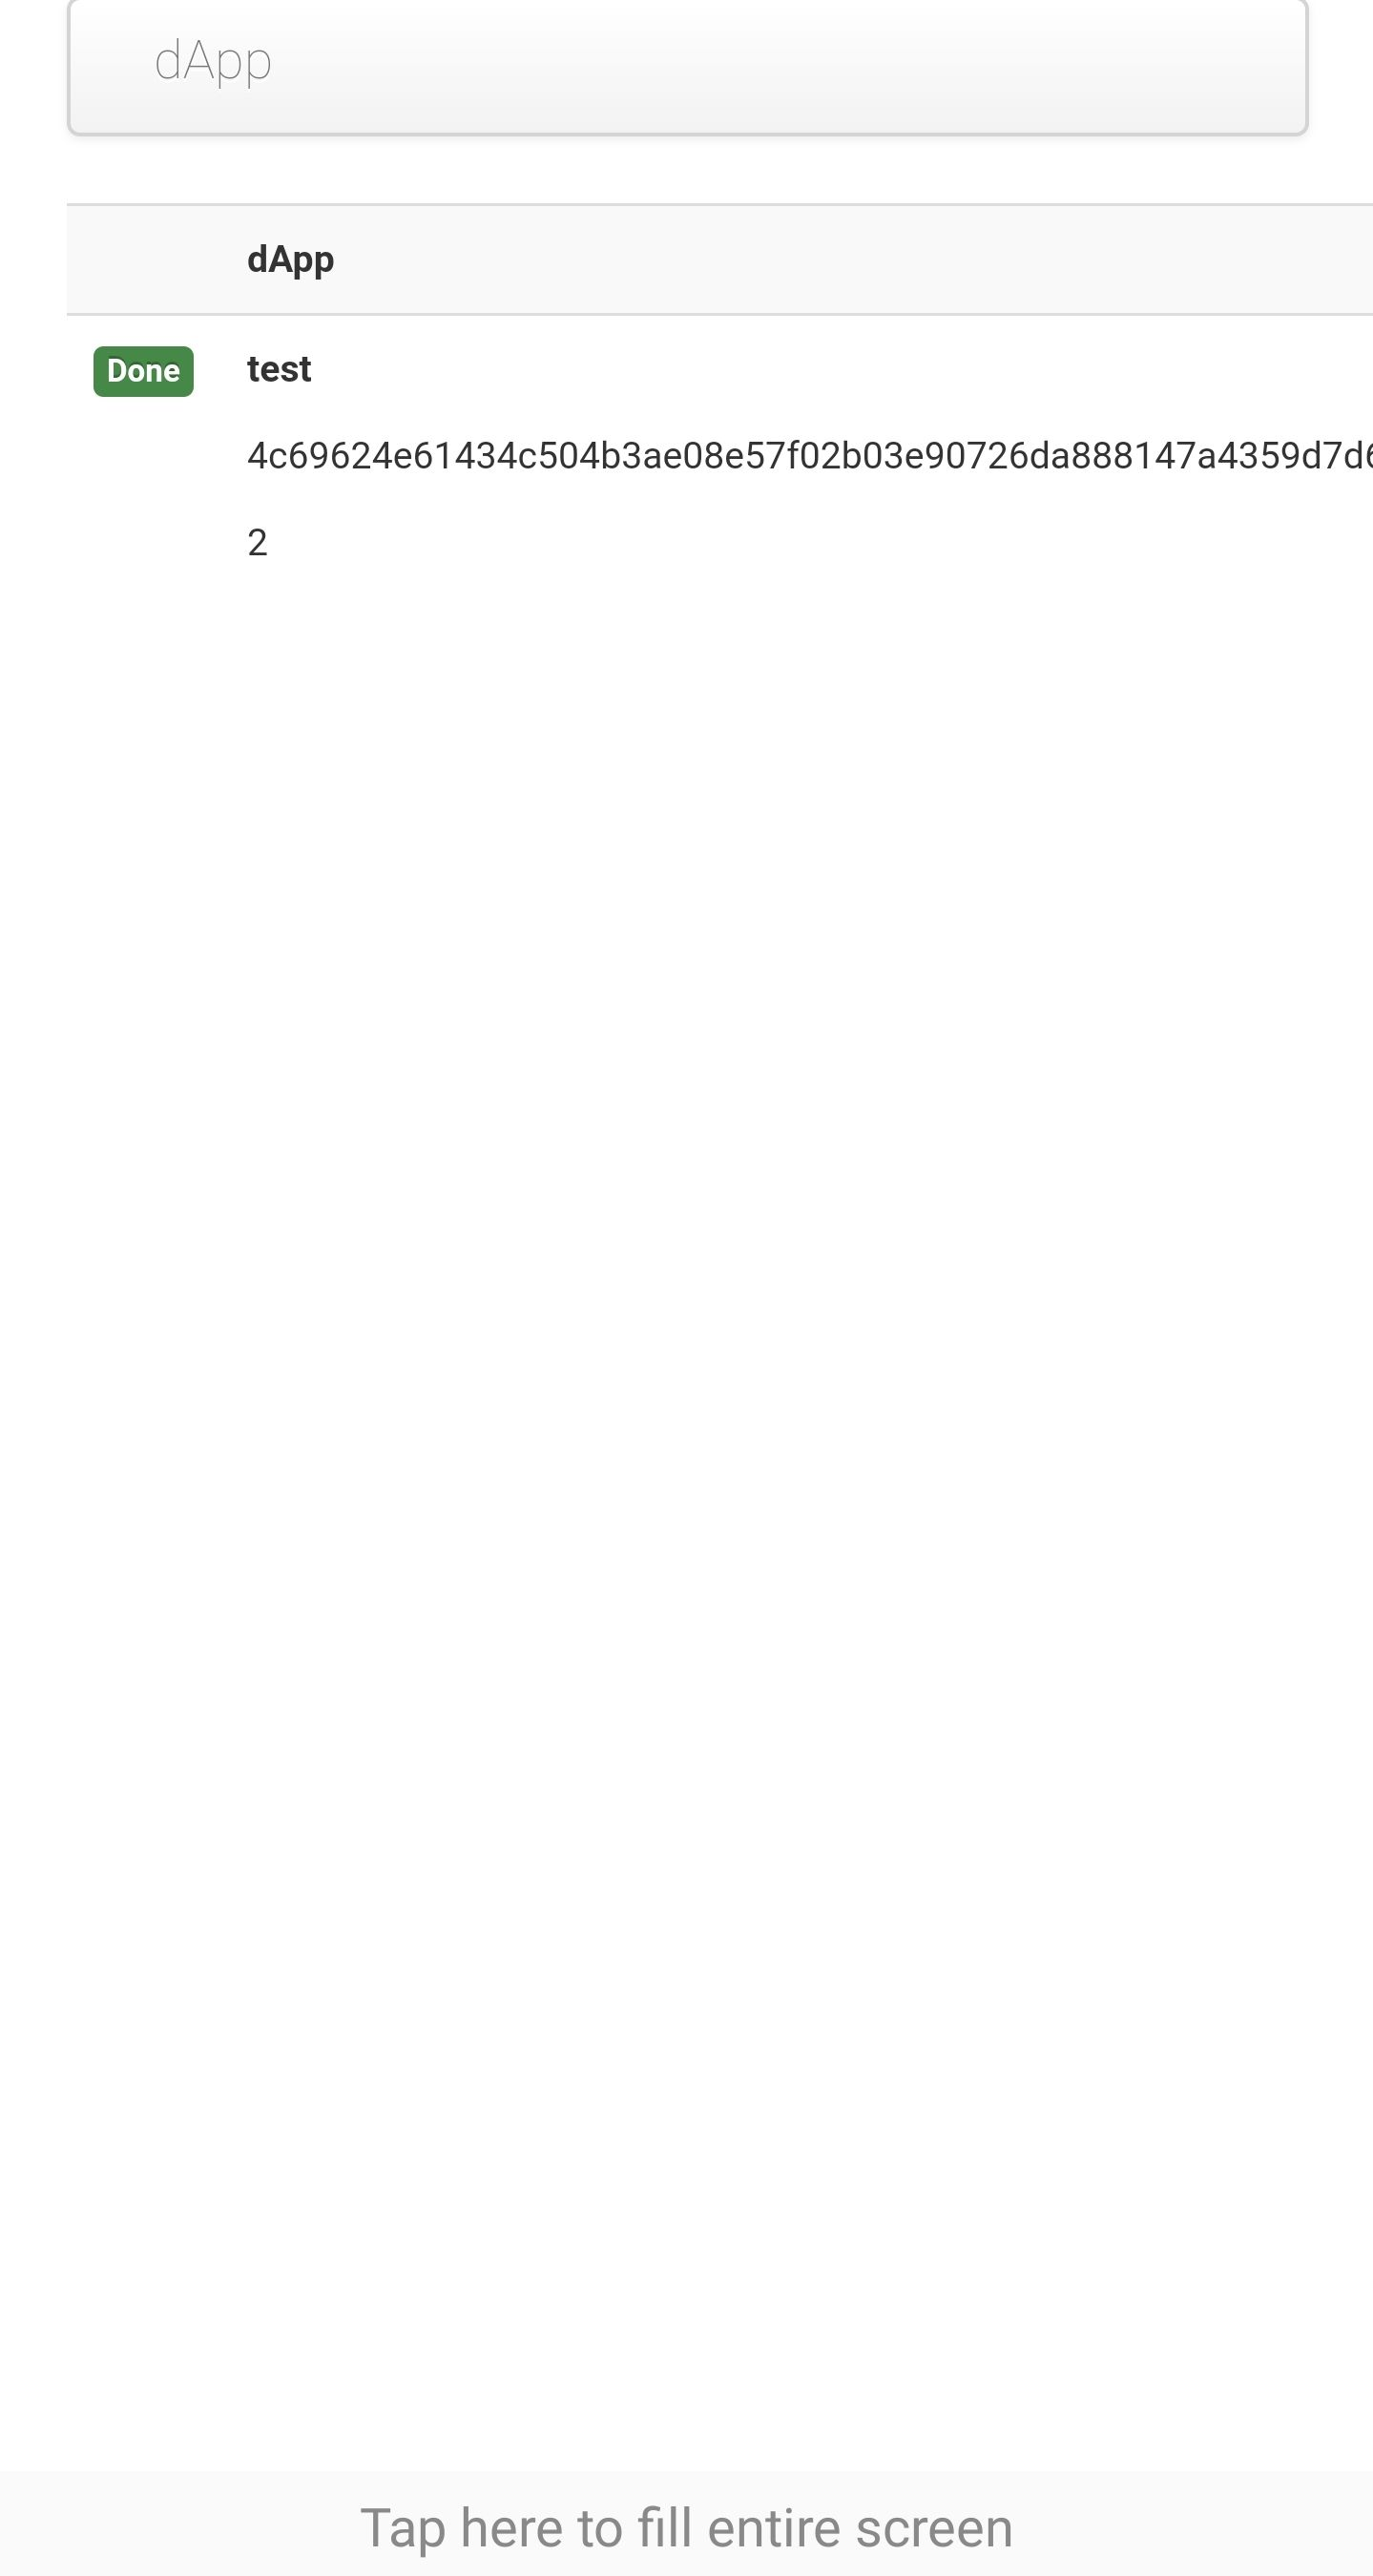
\includegraphics[width=0.5\textwidth]{images/android-app-screenshot.jpg}
%    \caption{\label{fig:android-app}}
%\end{figure}

\subsection{Efficient Cross-platform GUI}

\begin{figure*}[h!]
	\centering
	\begin{subfigure}[t]{.69\textwidth}
		\centering
		\captionsetup{width=.9\linewidth}
		{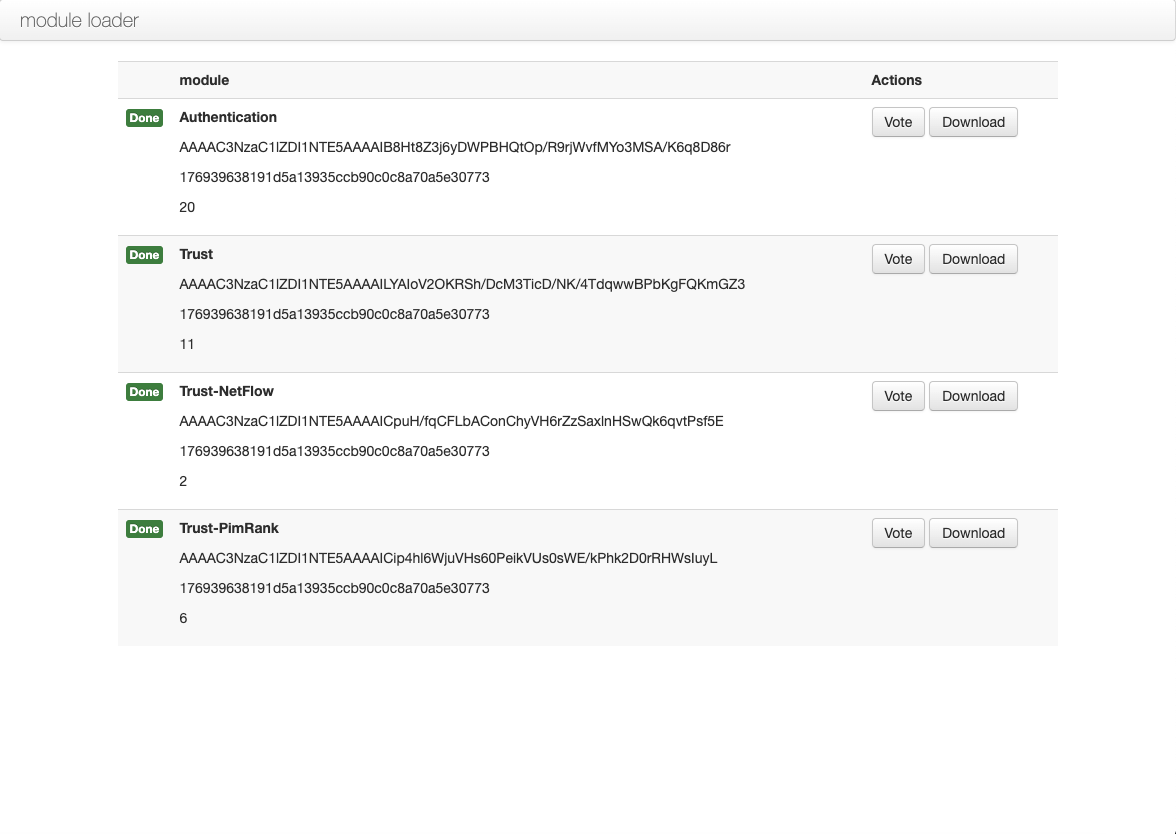
\includegraphics[width=0.95\linewidth]{images/gui-pc.png}}
		\caption{PC.}
		\label{fig:shared-library}
	\end{subfigure}\hfill%
	\begin{subfigure}[t]{.31\textwidth}
		\centering
		\captionsetup{width=.9\linewidth}
		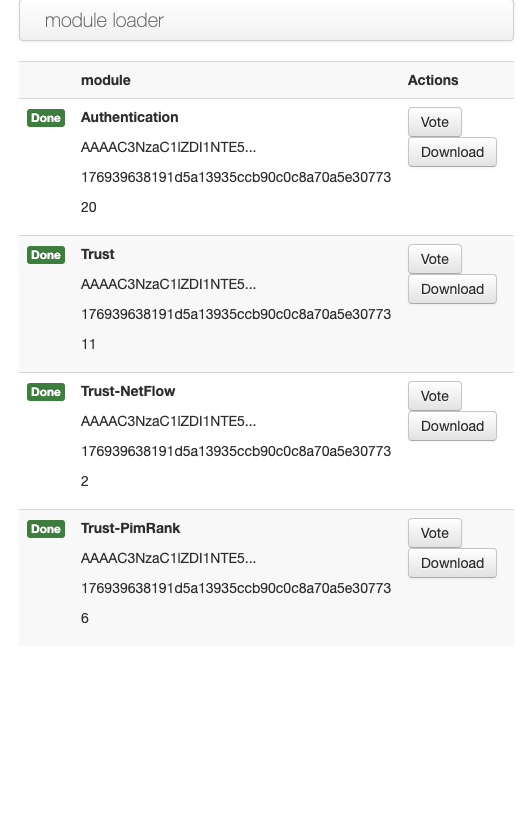
\includegraphics[width=0.95\linewidth]{images/gui-mobile.png}
		\caption{Mobile.}
		\label{fig:plugin}
	\end{subfigure}\vspace{0.5cm}\hfill%
	\caption{The graphical user interface of the FBase framework running on multiple device types.}
	\label{fig:evolution}
\end{figure*}

\newpage
		
\subsection{LOC Breakdown}

\begin{table}[ht!]
	\begin{tabular}{@{}llll@{}}
		\toprule
		&           & LOC    \\ \midrule
		FBase:   &           &        5029     \\
		& Discovery Protocol & 646    \\
		& Transport Mechanism& 140   \\
		& Runtime Engine    & 1134     \\
		Android: &           &  93285           \\
		& App       & 2157  \\ 
		& MP3 Package& 50584\\
		& MP3 Builder & 1722 \\ \bottomrule
	\end{tabular}
\end{table}

\subsection{Result Interpretation}

One part of evaluating FBase is testing if the concept works and is viable. Through the use of a non-trivial use-case, it was demonstrated that real-world practical problems can be solved using this framework.

The main advantage that the framework provided in the use-case was the introduction of modularity. On one hand, it has the benefit of flexibility and variety in use. On the other hand, modularization improves the manageability of maintenance for complex software like Tribler.

One of the disadvantages that followed from the use-case was the increased time that modules on FBase took to develop the application compared to implementing it in a monolithic architecture. A second more general disadvantage is that the module interconnect limits the complexity of the interaction between modules. This disadvantage did not limit the development of this use-case but changes the way applications need to be developed.

%allows complex software to be manageable for the purpose of maintenance

\section{Effectiveness of the Discovery Protocol}

%\subsection{Sensitivity Analysis}

One of the most important components of FBase is the module discovery protocol. To make this platform usable, this mechanism has to perform sufficiently effective without crippling the network with its overhead. The discovery protocol is compared to existing methods and the effectiveness is evaluated based on a theoretical sensitivity analysis.

\subsection{Existing Methods}

One of the simplest and easiest approaches that can be taken to discover new modules is flooding information packets throughout the network. This is the fastest approach for discovering modules, however, it will create a big strain on the network when then network becomes larger. It also allows malicious nodes to DDOS the network with relative ease.

Another approach is crawling. When crawling, nodes ask their neighboring nodes for the modules they have discovered. This approach is much less intensive on the global network as it works on a localized view. This method will eventually create a global coverage for module discovery, however, this method is very slow. Each module has to be propagated through each local view. This method is not suitable for large scale module discovery.

\subsection{Sensitivity Analysis}

FBase makes use of a discovery protocol based on a voting mechanism to prevent DDOSing while still being able to effectively discover new modules. It uses selective flooding on a local scale. Flooding is a effective way to reach a large number of nodes connected in a graph as can been seen in Figure~\ref{fig:discovery-flooding}. Even when there is a significant overlap in the neighbors of the nodes, thousands of nodes can be reached in very few steps.

\begin{figure}[ht!]
	\centering
	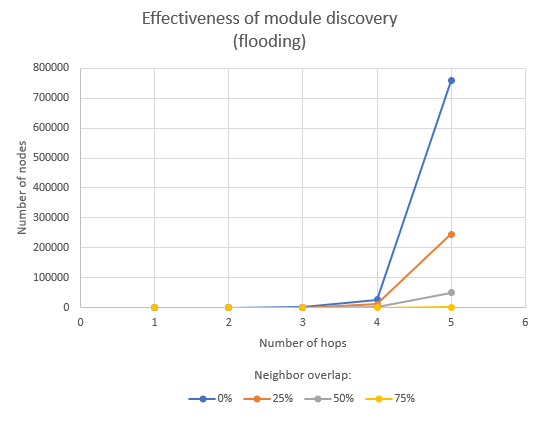
\includegraphics[width=0.64\textwidth]{images/evaluation-discovery-flooding.png}
	\caption{\label{fig:discovery-flooding} Effectiveness of module discovery (flooding).}
\end{figure}
%\begin{table}[h!]
%    \begin{tabular}{l|lllll}
%        \toprule
%        Neighbor overlap & 1     & 2      & 3        & 4           & 5              \\ \midrule
%        0\%              & 1 (0) & 31 (1) & 901 (31) & 26131 (901) & 757801 (26131) \\
%        25\%             & 1 (0) & 24 (1) & 530 (24) & 11662 (530) & 244904 (11662) \\
%        50\%             & 1 (0) & 16 (1) & 241 (16) & 3375 (241)  & 50385 (3375)   \\
%        75\%             & 1 (0)                      & 9 (1)  & 65 (9)   & 392 (65)    & 2289 (392) \\ \bottomrule   
%    \end{tabular}
%\end{table}

\newpage

However, If the same analysis is run with the voting mechanism the results are not as effective. The reason behind this behavior is that only a small fraction of all users will vote on a specific module. For this analysis, this percentage is set at 1\% of all nodes. Even in the most optimistic scenario where there is no neighbor overlap, the discovery stops after two steps with 24 nodes being aware of the module.

To circumvent this problem FBase uses the concept of Seed Discovery where multiple seed points are used for discovery when the author creates a module. This increases the chance for one of these starting points to overcome this barrier. This effect can be seen in Figure~\ref{fig:discovery-fbase-simple-0}. However, when applying Seed Discovery only when a module is created the discovery process still halts after 6 steps with 101 starting points.

\begin{figure}[ht!]
	\centering
	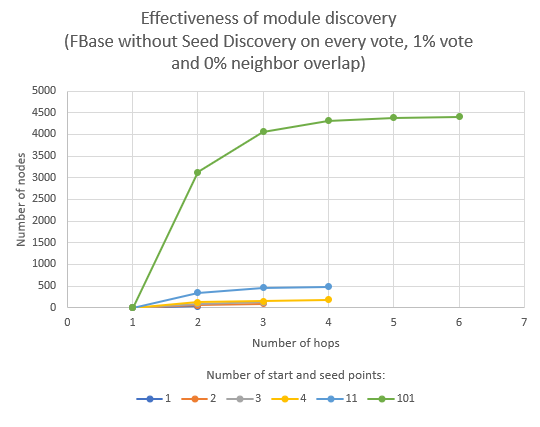
\includegraphics[width=0.64\textwidth]{images/evaluation-discovery-fbase-simple-0.png}
	\caption{\label{fig:discovery-fbase-simple-0} Effectiveness of module discovery (FBase without Seed Discovery on every vote, 1\% vote and 0\% neighbor overlap)}
\end{figure}

%1\% vote and 100\% disconnected
%\begin{table}[h!]
%    \begin{tabular}{@{}l|llllllll@{}}
%        \toprule
%        S & 1     & 2        & 3         & 4         & 5         & 6         & 7     \\ \midrule
%        1   & 1 (0) & 31 (1)   &     &        &           &           &               \\
%        2   & 1 (0) & 62 (1)   & 91 (2)    &     &      &           &               \\
%        3   & 1 (0) & 93 (1)   & 122 (2)   &    &        &           &               \\
%        4   & 1 (0) & 124 (1)  & 153 (2)   & 182 (3)   &    &       &               \\
%        ... &       &          &           &           &           &           &             \\
%        11  & 1 (0) & 341 (1)  & 457 (4)   & 486 (5)   &    &       &     \\
%         &       &          &           &           &           &           &     \\
%        101 & 1 (0) & 3131 (1) & 4059 (32) & 4320 (41) & 4378 (43) & 4407 (44) &  \\ \bottomrule
%    \end{tabular}
%\end{table}

In a more realistic scenario where there would be a 25\% overlap between the neighbors of nodes, the result would be even less effective as can be seen in Figure~\ref{fig:discovery-fbase-simple-25}.

\begin{figure}[ht!]
	\centering
	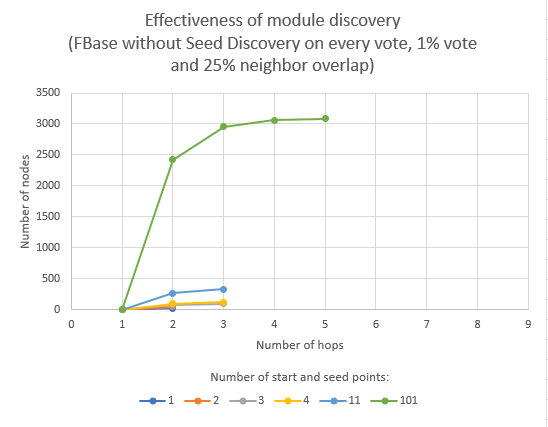
\includegraphics[width=0.64\textwidth]{images/evaluation-discovery-fbase-simple-25.png}
	\caption{\label{fig:discovery-fbase-simple-25} Effectiveness of module discovery (FBase without Seed Discovery on every vote, 1\% vote and 25\% neighbor overlap)}
\end{figure}

%1\% vote and 25\% disconnected
%\begin{table}[h!]
%    \begin{tabular}{@{}l|llllllll@{}}
%        \toprule
%        S & 1     & 2        & 3         & 4         & 5         & 6         & 7     \\ \midrule
%        1   & 1 (0) & 24 (1)   &     &        &           &           &               \\
%        2   & 1 (0) & 48 (1)   &     &     &      &           &               \\
%        3   & 1 (0) & 72 (1)   & 94 (2)   &    &        &           &               \\
%        4   & 1 (0) & 96 (1)  & 118 (2)   &    &    &       &               \\
%        ... &       &          &           &           &           &           &             \\
%        11  & 1 (0) & 264 (1)  & 330 (4)   &    &   &       &     \\
%        ... &       &          &           &           &           &           &     \\
%        101 & 1 (0) & 2424 (1) & 2952 (25) & 3062 (30) & 3084 (31) &  &  \\ \bottomrule
%    \end{tabular}
%\end{table}

\newpage

When the Seed Discovery is applied on every vote, a continuous discovery can be found with 11 starting points as can be seen in Figure~\ref{fig:discovery-fbase-extended-25}.

\begin{figure}[ht!]
	\centering
	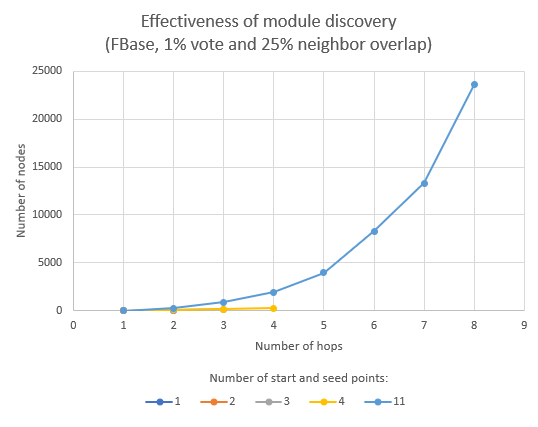
\includegraphics[width=0.64\textwidth]{images/evaluation-discovery-fbase-extented-25.png}
	\caption{\label{fig:discovery-fbase-extended-25} Effectiveness of module discovery (FBase without Seed Discovery on every vote, 1\% vote and 25\% neighbor overlap)}
\end{figure}

%1\% vote and 25\% disconnected and direct random discovery
%\begin{table}[h!]
%    \begin{tabular}{@{}l|llllllllll@{}}
%        \toprule
%        S & 1     & 2        & 3         & 4         & 5         & 6         & 7   & 8 & 9  \\ \midrule
%        1   & 1 (0) & 24 (1)   &     &        &           &           &      & &         \\
%        2   & 1 (0) & 48 (1)   &    &     &      &           &         & &      \\
%        3   & 1 (0) & 72 (1)   & 142 (2)(1)   &    &        &           &      & &         \\
%        4   & 1 (0) & 96 (1)  & 166 (2)(1)  & 236 (3)(2)   &    &       &     & &          \\
%        ... &       &          &           &           &           &           &      & &       \\
%        11  & 1 (0) & 264 (1)  & 882 (4)(3)   & 1912 (9)(8)  &  3972 (19)(18)  &  8298 (40)(39)     &  13292 (83)(61) &  23592 (133)(111) & ... \\ \bottomrule
%    \end{tabular}
%\end{table}

This approach results in an effective discovery without flooding the network and preventing malicious attempts.

%\section{Requirement Assessment}
%
%To evaluate FBase as a concept, the individual parts that make up the framework need to be evaluated and see if they conform to the requirements set in Chapter 2.
%
%\begin{itemize}[nosep]
%    \item Testing if the concept works and is viable.
%    \item Examining the effectiveness of the discovery protocol% and the module communication.
%\end{itemize}

\subsection{Result Interpretation}

The effectiveness of the discovery protocol is the second part that was analyzed in this evaluation. The sensitivity analysis indicated that a degree of flooding is necessary to accomplish effective network coverage without putting excessive strain on the network. When comparing different situations of selective flooding by introducing voting, it was shown that seed discovery is necessary on every vote for the discovery to reach global coverage.


\chapter{Conclusion}

%% bibliography
\renewcommand\bibname{References}
\bibliography{references}

    %% Use letters for the chapter numbers of the appendices.
\appendix
    %\chapter{Module tutorial}
    
% This document assumes you have installed all of the dependencies as instructed in the README.md. You will learn how to set up the framework and create your first module.
% 
% \section{Files}
% 
% First we will setup a working directory to run the framework in. This tutorial will place all of its files in the ~/Documents/module\_tutorial directory. You are free to choose whatever directory you want, to place your files in.
% 
% In the working directory, we will now clone FBase through git:
% \begin{lstlisting}
% git clone https://github.com/mitchellolsthoorn/ipv8-module-loader.git
% \end{lstlisting}
% 
% You should see a folder called \textit{ipv8-module-loader} appear in the working directory.
% 
% At the end of this setup step you should have the following files in your working directory:
% 
% (folder) pyipv8
% (file) __init__.py
% (file) main.py
    \newpage\null\thispagestyle{empty}\newpage

\end{document}